%generare il pdf con il comando: pdflatex main.tex
\documentclass[a4paper, oneside, openany,12pt]{article}
\usepackage{graphbox}
% permette di modificare i margini
\usepackage[top=3.1cm, bottom=3.1cm, left=2.2cm, right=2.2cm]{geometry}
\usepackage{lastpage} %info sul # dell'ultima pagina del documento
\usepackage{fancyhdr} %per modificare dimensioni,margini, intestazioni e righe a piè di pagina

\usepackage[htt]{hyphenat}

\fancypagestyle{plain}{
  % cancella tutti i campi di intestazione e piè di pagina
  \fancyhf{}
  
  \rhead{\sectiontitle}
  
  \rfoot{Page \thepage{} di \pageref{LastPage}} %es: pag: 4 di 10

  %linea orizzontale alle posizioni top e bottom della pagina
  \renewcommand{\headrulewidth}{0.2	pt}  
  \renewcommand{\footrulewidth}{0.2pt}
}
\pagestyle{plain}

%Comando Spazio
\newcommand{\Spazio}{\mbox{} \\ \mbox{} \\ }  


%\usepackage{calc} %introduce la notazione infissa per le op. aritmetiche interne a LaTeX

\usepackage[utf8]{inputenc}
\usepackage[T1]{fontenc}
\usepackage[english]{babel} %il documento è in inglese
%\usepackage{textcomp} %The pack­age sup­ports the Text Com­pan­ion fonts, which pro­vide many text sym­bols
%(such as baht, bul­let, copy­right, mu­si­cal­note, onequar­ter, sec­tion, and yen), in the TS1 en­cod­ing.

\usepackage{graphicx}       %permette di inserire delle immagini
\usepackage{caption}        %numerazione figure e loro descrizione testuale
\usepackage{subcaption}     %sottofigure numerabili
\usepackage{float}  %permette di inserire un # qualsiasi di figure fluttuanti
\usepackage{xcolor}
\usepackage{color, colortbl}
\usepackage{rotating} %permette di ruotare le immagini
%\usepackage{changepage} %utile se c'è bisogno di aggiustare margini per centrare figure

%package utili per la math mode ( $ ... $ o \[ ... \] )
\usepackage{amsmath}
\usepackage{amssymb}
\usepackage{amsfonts}
%\usepackage{euler}    %font 'ams euler', lo stesso di 'Concrete Mathematics' di Knuth
\usepackage{amsthm}
\usepackage{mathtools}

% package utili per tabelle(\thead in particolare)
\usepackage{array, booktabs, caption}
\usepackage{makecell}
\renewcommand\theadfont{\bfseries}
\usepackage{boldline}

\usepackage{listings} %permette di inserire degli spezzoni di codice

\usepackage{tikz} %disegno di immagini vettoriali a schermo. Utile per grafi
\usetikzlibrary{arrows.meta}
\usetikzlibrary{graphs}
\usetikzlibrary{arrows}
%\usepackage{tikz-uml} %serve per disgnare l'UML, fantastica guida:
%https://perso.ensta-paristech.fr/~kielbasi/tikzuml/var/files/doc/tikzumlmanual.pdf
%download package: http://perso.ensta-paristech.fr/~kielbasi/tikzuml/

%package per le tabelle
\usepackage{booktabs} %permette di poter usare delle liste nelle tabelle
\usepackage{tabularx} 
\usepackage{longtable} %una tabella può continuare su più pagine
\usepackage{multirow} %utile per visualizzare una cella su più righe
%\usepackage{multicolumn} %cella su più colonne
%\usepackage[table]{xcolor} %rende disponibile l'utilizzo di un colore per lo sfondo
                        %delle celle di una tabella

%crea una cella per le tabelle in grado di andare a capo con \newline
%https://tex.stackexchange.com/questions/12703/how-to-create-fixed-width-table-columns-with-text-raggedright-centered-raggedlef
\usepackage{array}
\newcolumntype{L}[1]{>{\raggedright\let\newline\\\arraybackslash\hspace{0pt}}m{#1}}
\newcolumntype{C}[1]{>{\centering\let\newline\\\arraybackslash\hspace{0pt}}m{#1}}
\newcolumntype{R}[1]{>{\raggedleft\let\newline\\\arraybackslash\hspace{0pt}}m{#1}}


%indice con i puntini
\usepackage{tocloft}
\renewcommand\cftsecleader{\cftdotfill{\cftdotsep}}

%Pacchetto per i colori delle tabelle
\usepackage{color, colortbl}

%http://ctan.mirror.garr.it/mirrors/CTAN/macros/latex/contrib/appendix/appendix.pdf
\usepackage{appendix} %aggiunge dei comandi per l'appendice
\usepackage{parskip} %aiuta LaTeX a trovare il miglior stile per i page break
\setcounter{secnumdepth}{5} % numera i sottoparagrafi
\setcounter{tocdepth}{5} %aggiunge all'indice i sottoparagrafi
%\usepackage{titlesec} %\begin{paragraph} si può usare come subsubsubsection!


\usepackage{breakurl}%\url{...} può continare alla linea successiva. (si può andare a capo)

\definecolor{Maroon}{cmyk}{0, 0.87, 0.68, 0.32}
\usepackage[colorlinks=true]{hyperref}
\hypersetup{
    colorlinks=true,
    citecolor=black,
    filecolor=black,
    linkcolor=black, % colore dei link interni
    urlcolor=blue  % colore dei link interniesterni
}

%impostazioni per il codice che deve finire dentro a
%\begin{lstlisting}

\definecolor{listinggray}{gray}{0.9}
\definecolor{lbcolor}{rgb}{0.9,0.9,0.9}
\lstset{
backgroundcolor=\color{lbcolor},
    tabsize=4,    
%   rulecolor=,
    language=[GNU]C++,
    basicstyle=\scriptsize,
    upquote=true,
    aboveskip={1.5\baselineskip},
    columns=fixed,
    showstringspaces=false,
    extendedchars=true,
    inputencoding=utf8,
    breaklines=true,
    prebreak = \raisebox{0ex}[0ex][0ex]{\ensuremath{\hookleftarrow}},
    frame=single,
    numbers=left,
    showtabs=false,
    showspaces=false,
    showstringspaces=false,
    identifierstyle=\ttfamily,
    keywordstyle=\color[rgb]{0,0,1},
    commentstyle=\color[rgb]{0.026,0.112,0.095},
    stringstyle=\color[rgb]{0.627,0.126,0.941},
    numberstyle=\color[rgb]{0.205, 0.142, 0.73},
%        \lstdefinestyle{C++}{language=C++,style=numbers}’.
}
\lstset{
  backgroundcolor=\color{white},
  tabsize=4,
  language=C++,
  captionpos=b,
  tabsize=3,
  frame=lines,
  numbers=left,
  numberstyle=\tiny,
  numbersep=5pt,
  breaklines=true,
  showstringspaces=false,
  basicstyle=\footnotesize,
  identifierstyle=\color{black},
  keywordstyle=\color[rgb]{0,0,1},
  commentstyle=\color{gray},
  stringstyle=\color{red}
}
% Creazione della copertina
\newcommand{\copertina}{
  \newgeometry{top=5cm}
  
  \begin{titlepage}
  \begin{center}
 
	\begin{tikzpicture}[remember picture, overlay, scale=.5, transform shape, opacity=0.15]
		\node[anchor=center] at (current page.west){%
		\pgfimage{Style/logo.png}};
	\end{tikzpicture}
    
  \vspace{1cm}

  \begin{Huge}
    \textbf{Web Information Management}\\
    \vspace{20pt}  
    \textbf{Usability analysis:} \\
    \textbf{Sicilian Goodness} \\
  \end{Huge}

  \vspace{9pt}  
  
  \begin{large}
  	\today
  \end{large}	  
  
  \vspace{15pt}
  
  \vspace{15pt}

  \begin{center}
  	
  	\begin{tabular}{ c c }
		\textbf{Budai Matteo} & 2057217  \\
  	\end{tabular}
  	
  \end{center}

  \end{center}
  \end{titlepage}
  
  \restoregeometry
}

\newcommand{\code}[1]{\flextt{\texttt{#1}}}

\newcommand{\gl}[1]{\textit{#1}\ped{g}}

\newcommand{\sectiontitle}{}



\begin{document}
\copertina
\tableofcontents
\pagebreak

%\listoffigures
%\listoftables

% Comando per testare con le linee più grosse
\arrayrulewidth=1pt
% Colori per la tabella
\definecolor{title_row}{rgb}{0.13, 0.59, 0.95}
\definecolor{title_text}{rgb}{1, 1, 1}

% SEZIONI DEL DOCUMENTO
% qui vanno presentate in ordine di apparizione le sezioni che compongono il documento
\section{Introduction}

This report is based on the usability analysis of the site \url{https://www.siciliangoodness.com/}.
The web site is an italian web site that allows you to see and buy Sicilian products. \newline

	\begin{figure}[H]
	\centering
\includegraphics[width=9cm]{Img/logo.jpg}
	\caption{Sicilian Goodness Logo}
	\end{figure}

Sicilian Goodness is the name and brand of a young and dynamic Sicilian company, an innovative startup founded in September 2015 by 2 young entrepreneurs from Palagonia, Sebastiano Azzolina and Vanessa Auteri, towards a project to export the products of their land. \newline 

Its purpose is to expand the brand through the opening of franchised stores and bring Sicilian cuisine and products ever closer to consumers, for example in Veneto. \\


\pagebreak

\section{Preliminary analysis}

\subsection{Context}
Sicilian Goodness is a web site specialized in the sale and export of Sicilian products.
Its scope is very specific and for this reason only those who are interested will explore this site. 

\subsection{Structure}
To ensure a good level of usability, a website must be developed according to a well-considered structure, in order to make it logical and predictable. The site has a banal structure, with a homepage that leads to several other pages containing different options. It is therefore intuitive to any user understand how to use the interface at a basic level and navigate in the site.

\subsection{Domain name}
The name is a very important factor. \newline
\textbf{Sicilian Goodness} (sicialiangoodness.com) is:
\begin{itemize}
	\item unique;
	\item contains '.com' (impact: +45\%);
	\item easy to memorize and write;
	\item uses existing words (in English too);
	\item not use dashes.
\end{itemize}

Even if the name is not short, in the overall the domain name passes most of the guidelines.


\pagebreak
\section{Homepage}

\subsection{General description}
The homepage analysis of \url{https://www.siciliangoodness.com/} is performed with many screens since it is developed vertically.

	\begin{figure}[H]
	\centering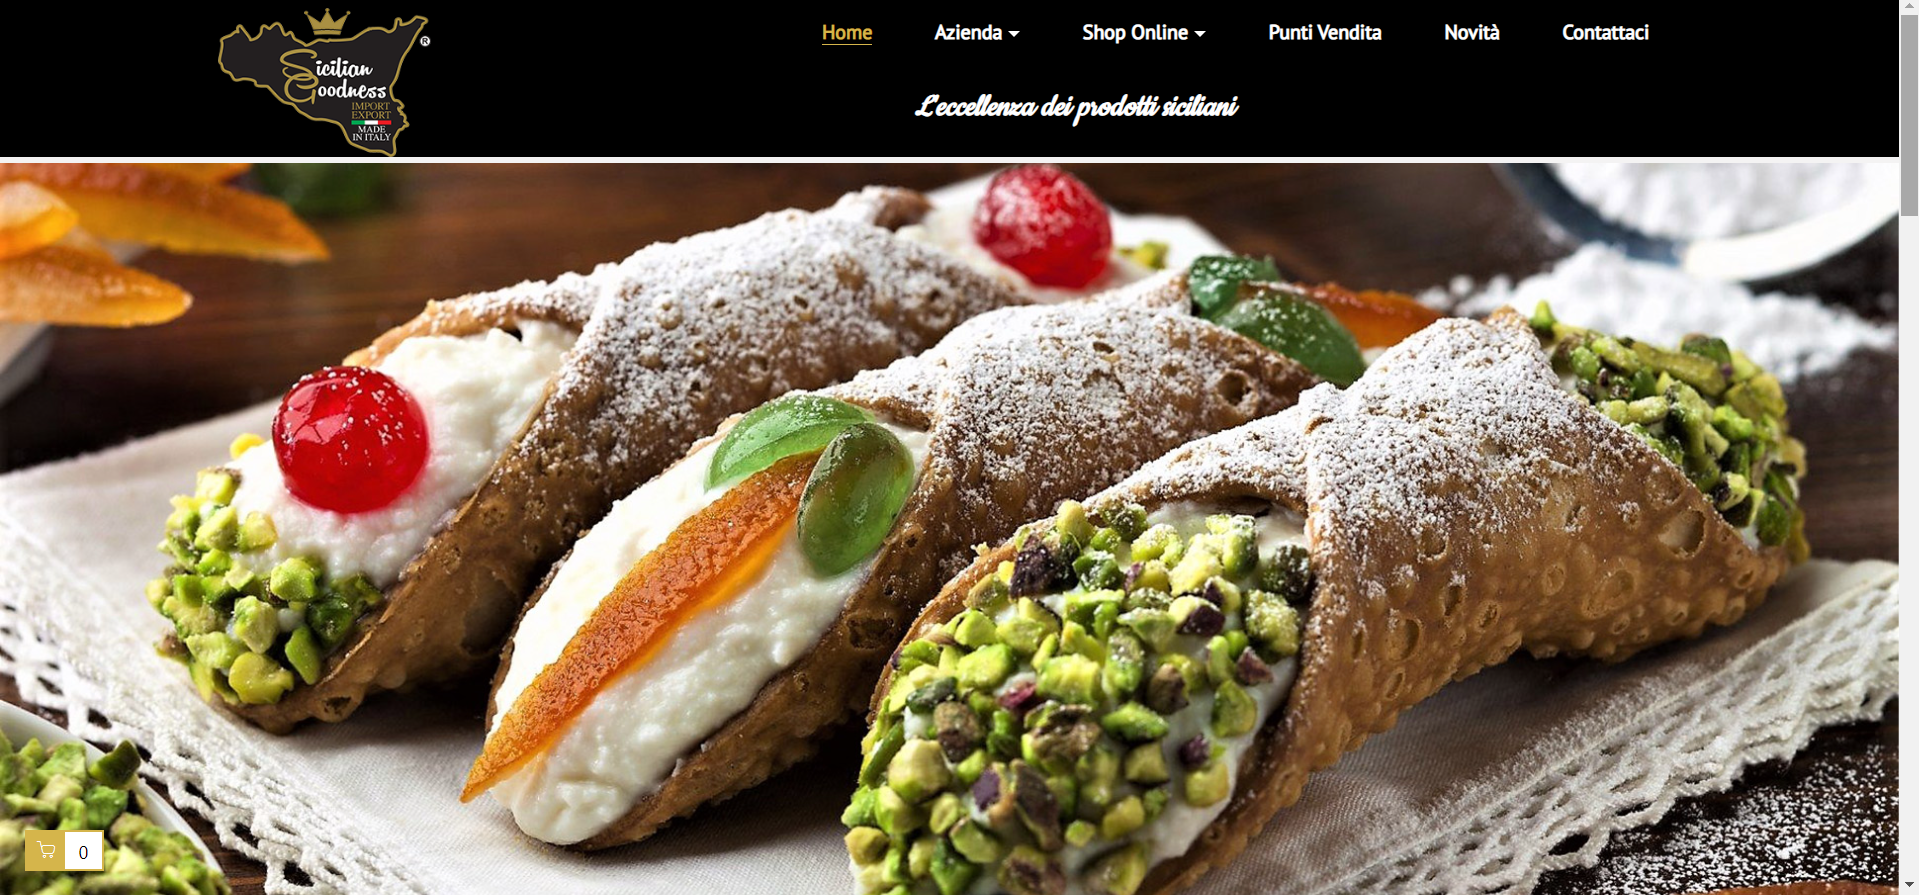
\includegraphics[width=12cm]{Img/hom1.png}
	\caption{Homepage 1}
	\end{figure}

The most important part of the homepage, visible without scrolling. They can be noticed some important and recurring elements on websites, such as:

\begin{itemize}
	\item the logo is well-suited in the top-left corner;
	\item the breadcrumb for the navigation;
	\item the colors are used well (white and black, readable).
\end{itemize}

As we can see in the images below we have a problem with the images of the homepage which are constantly changing. 
Even if today this is a common practice, the changing of the images can confuse the users.
Especially in the \hyperlink{hom5}{Figure 6}, the products seem to be clickable but they are not, so the visual metaphore is not respected. \newline

\begin{figure}[H]
	\centering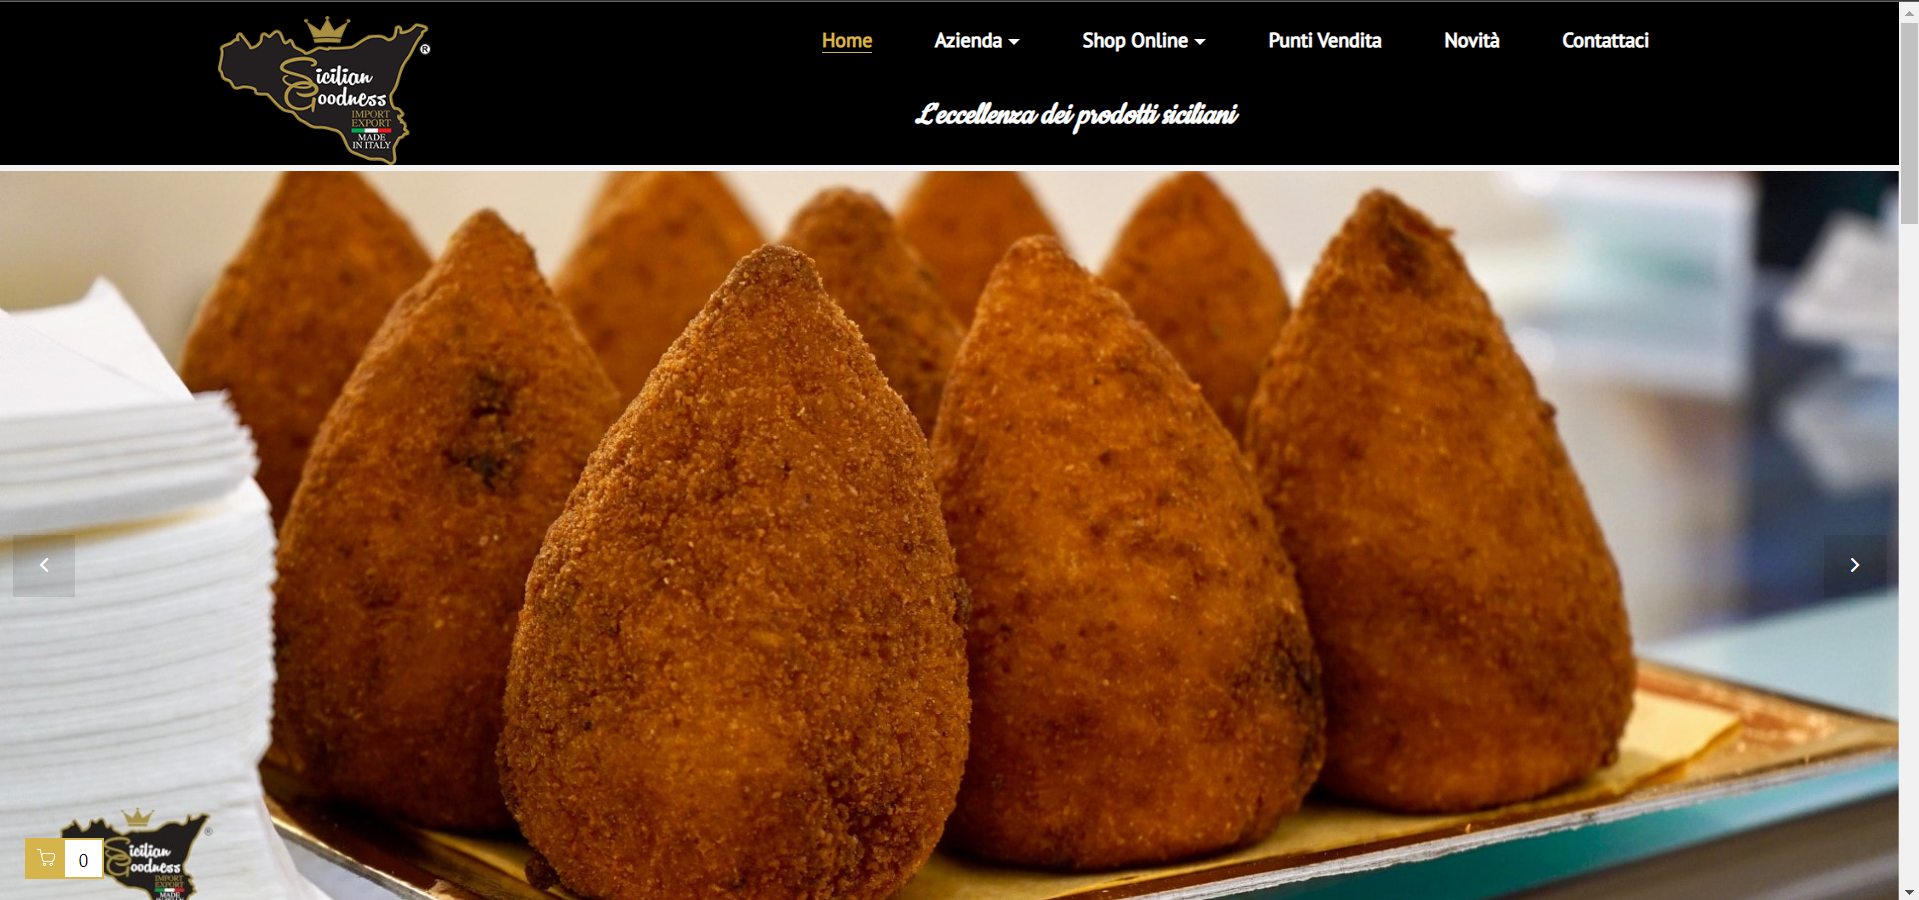
\includegraphics[width=12cm]{Img/hom2.png}
	\caption{Homepage 2}
\end{figure}

\begin{figure}[H]
	\centering
\includegraphics[width=12cm]{Img/hom3.png}
	\caption{Homepage 3}
\end{figure}

\begin{figure}[H]
	\centering
\includegraphics[width=12cm]{Img/hom4.png}
	\caption{Homepage 4}
\end{figure}

\begin{figure}[H]
	\label{hom5}
	\centering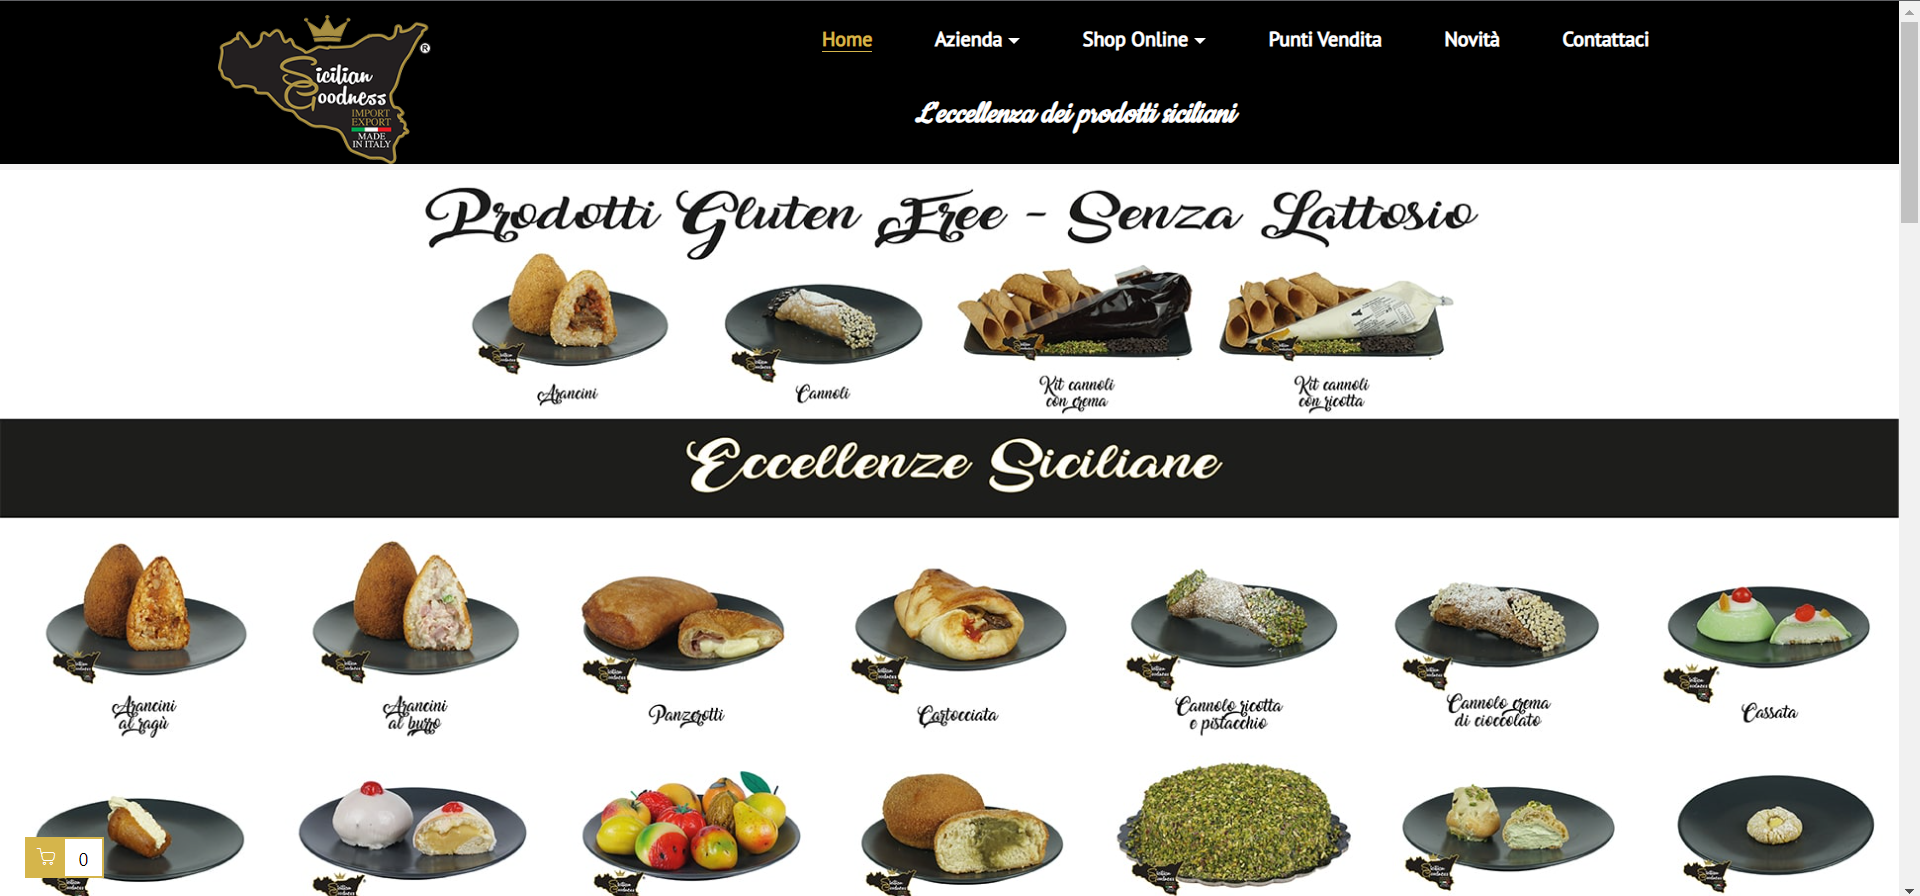
\includegraphics[width=12cm]{Img/hom5.png}
	\caption{Homepage 5}
\end{figure}

\pagebreak

In the following two scrolls we have the content of the page.

\begin{figure}[H]
	\centering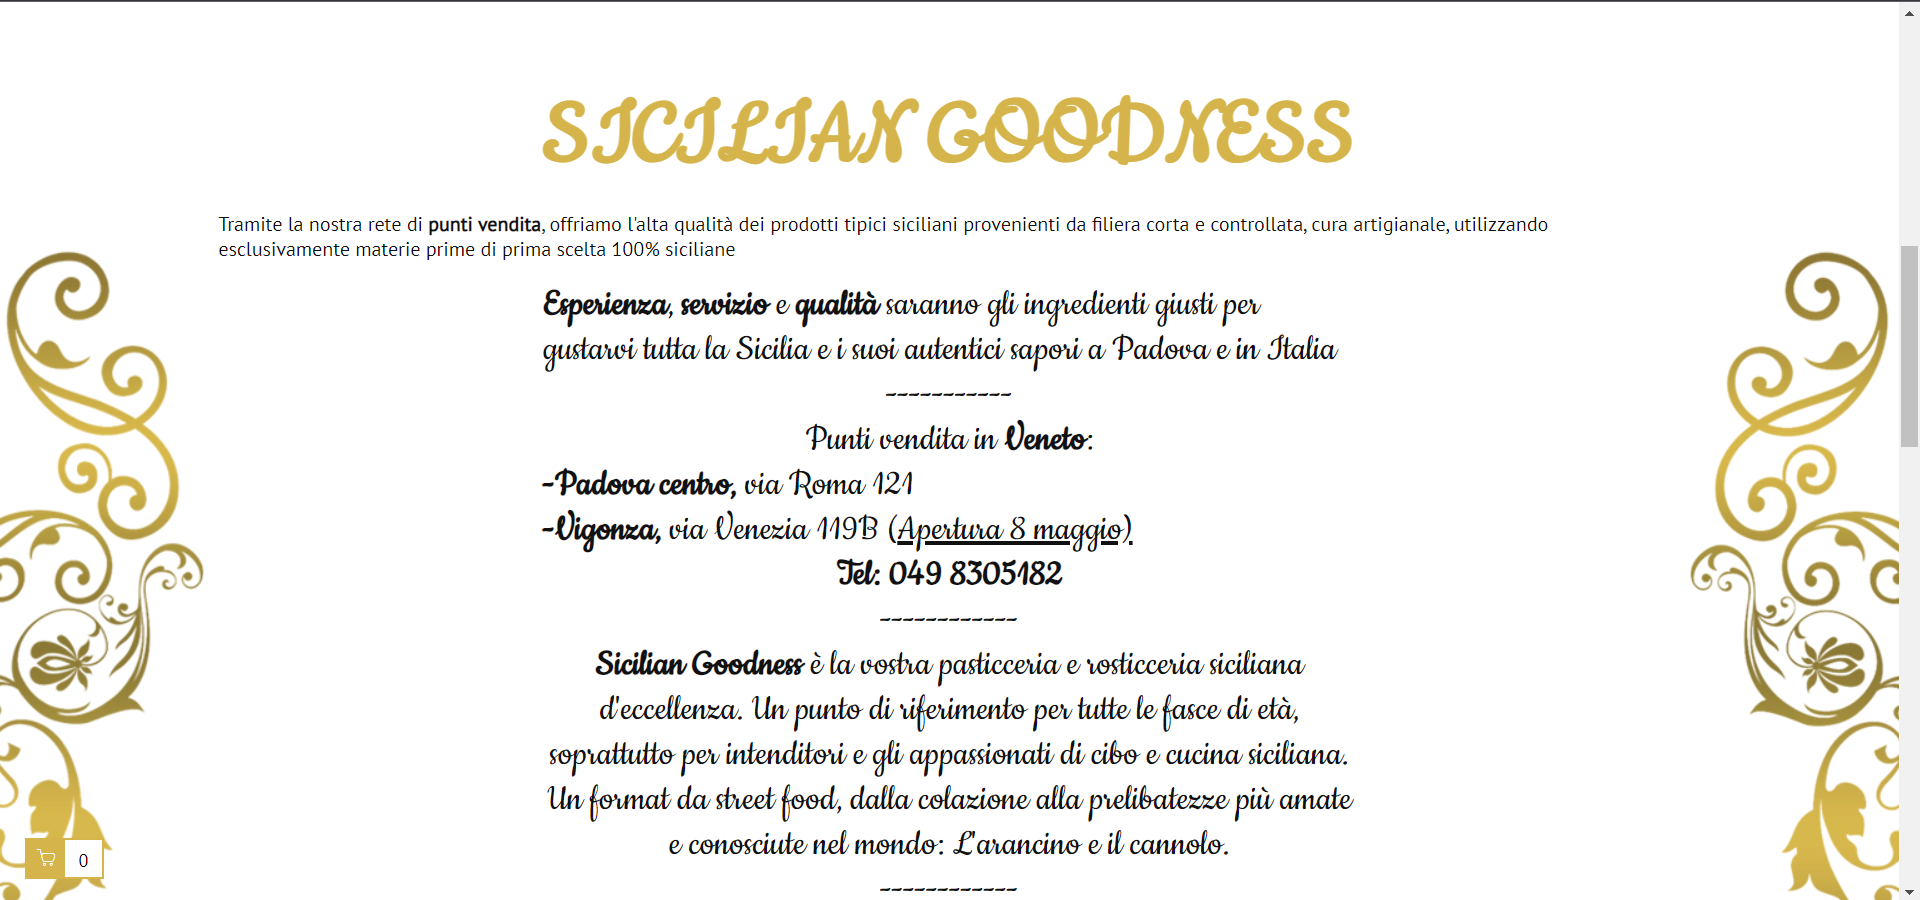
\includegraphics[width=12cm]{Img/content1.png}
	\caption{Content 1}
\end{figure}

\begin{figure}[H]
	\centering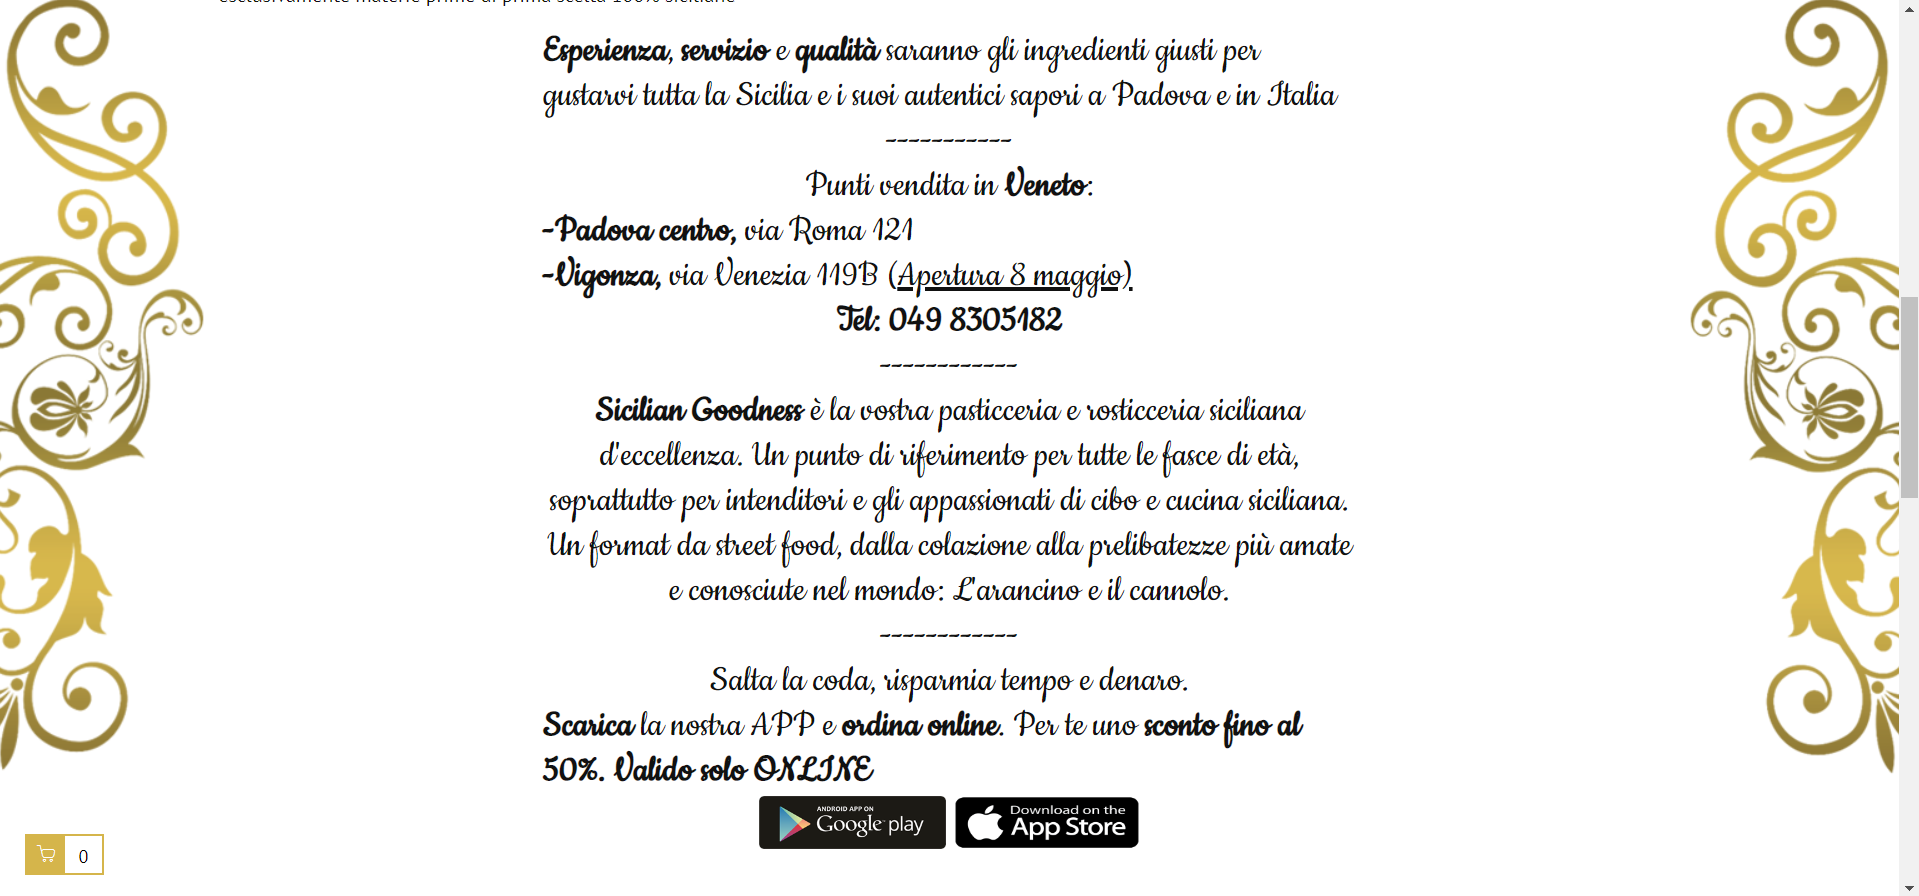
\includegraphics[width=12cm]{Img/content2.png}
	\caption{Content 2}
\end{figure}

The footer include all the information about the company.

\begin{figure}[H]
	\centering
\includegraphics[width=12cm]{Img/contacts.png}
	\caption{Footer}
\end{figure}


\subsection{The Six Ws}
The best way to evaluate the impact of the homepage is to analyze the so-called "Six Ws".

\subsubsection{Where?}

Question: \textit{Where did I (user) arrive?}
\newline
A user who arrives on the site for the first time immediately understands that it is on a site connected to the kitchen. Name and logo help the user to understand where he is. Indeed the user immediately understande that he is on a site that offers Sicilian products. After seeing the pictures and reading the text, the user understand perfectly where he is.

\begin{figure}[H]
	\centering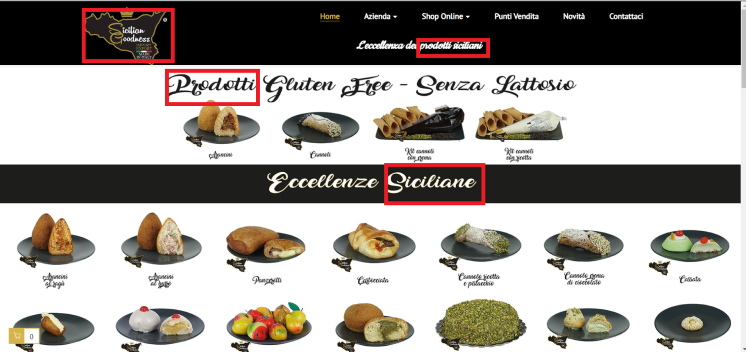
\includegraphics[width=12cm]{Img/where1.png}
	\caption{Where 1}
\end{figure}

\begin{figure}[H]
	\centering
\includegraphics[width=12cm]{Img/where2.png}
	\caption{Where 2}
\end{figure}

\pagebreak

\subsubsection{Who?}

Question: \textit{Who is behind the website?}
\newline
The identity of the creator/owner of the site is not totally clear. Certainly the logo helps to identify it if you already know it, however for a user who has never heard of the site, the author is unknown and probably it will remain so. Indeed, to find some information about it, it is necessary scroll to the bottom of the page, until
to arrive in the footer, where the owner is written in a very small font, Sicilian Goodness srl. In addition, 'Azienda' and 'Parlano di noi' are two links that point to a page that offers some additional information the company.
An other way is to click on 'Azienda' and 'Contattaci' in the top of the homepage. For these reasons, the Who axis is not well specified, as it takes too long to find an answer, which the user does not have and which can lead to increased dissatisfaction.

\begin{figure}[H]
	\centering
\includegraphics[width=12cm]{Img/who.png}
	\caption{Who}
\end{figure}

\subsubsection{Why?}

Question: \textit{What are the benefits? Why should I stay?}
\newline
The site specified very well why the user should stay in the website. In fact, the word 'Eccelenze' is repeated multiple times in the homepage.
In addition, as we can see in the image below, the site give a short description to persuade the user to stay.
\begin{figure}[H]
	\centering
\includegraphics[width=12cm]{Img/why.png}
	\caption{Why}
\end{figure}

\pagebreak

\subsubsection{What?}

Question: \textit{What choices do I have?}
\newline
As before, the homepage is strongly oriented towards the content, which is proposed several times and in different ways. The main navigation menu presents several items that recall what the site offers. We understand immediately that this is an e-commerce to buy or order products online.

\subsubsection{When?}

Question: \textit{What are the last news?}
\newline
The When axis is clearly specified. Indeed in the navigation menu we have the section 'Novità'.
In addition, as we can see in the image below, the website offers in the homepage an appropriate section for the news.

\begin{figure}[H]
	\centering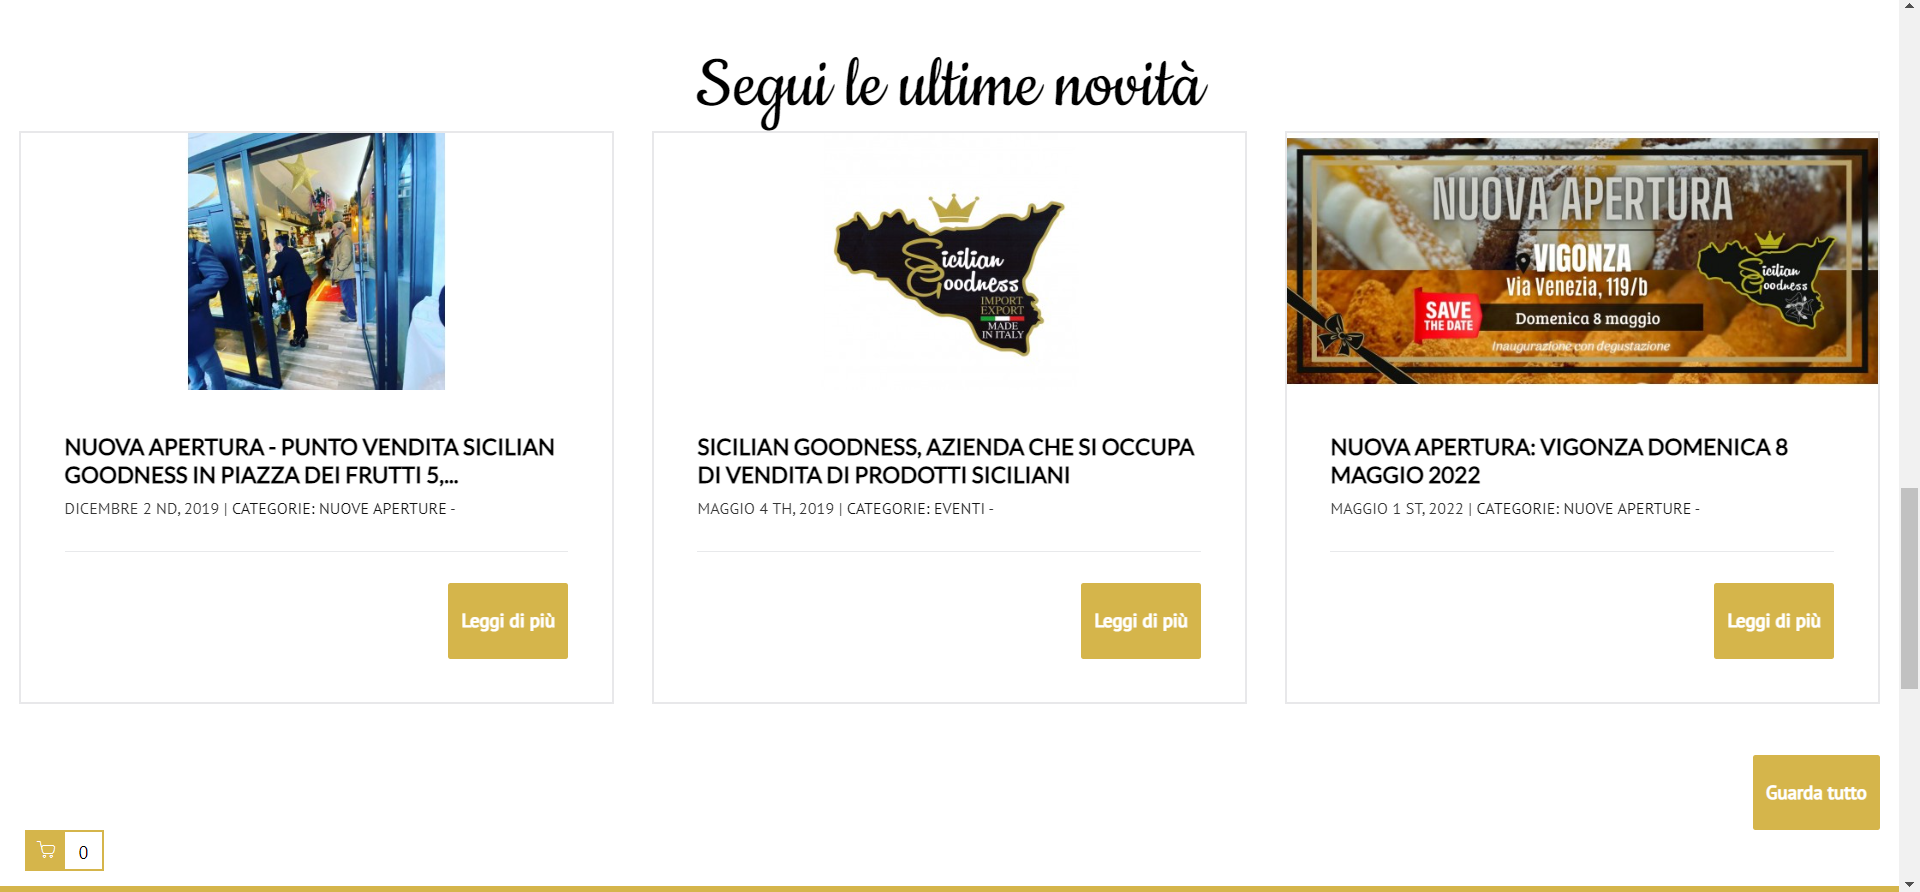
\includegraphics[width=12cm]{Img/news.png}
	\caption{When}
\end{figure}

\subsubsection{How?}

Question: \textit{How do I arrive where I want?}
\newline
The homepage offers a main menu to reach the page that the user wants. The main menu is well specified in the top if the page.

\begin{figure}[H]
	\centering
\includegraphics[width=12cm]{Img/how.png}
	\caption{How}
\end{figure}

\paragraph{Menu}
The menu presents the following items: 
\begin{itemize}
	\item Home: It's a link that reloads the website;
	\item Azienda: The underlying menu points to various pages that describe the company;
	\item Shop Online: The underlying menu points to the page where you can see the products and buy it;
	\item Punti Vendita: It points to a page that gives a description of the stores of the company, how to reach its and some useful information;
	\item Novità: It points to a page that provide all the news of the company;
	\item Contattaci: It points to a page with the contacts of the company.
\end{itemize}

\begin{figure}[H]
	\centering
\includegraphics[width=12cm]{Img/menu.png}
	\caption{Menu 1}
\end{figure}

The voice 'Azienda' offers the following items:
\begin{itemize}
	\item Chi siamo: It provides a description of the company and how it has evolved over time;
	\item Qualità: It provides a description of the quality of the products and how they are processed;
	\item Franchising: It provides a description about the franchising.
\end{itemize}

\begin{figure}[H]
	\centering
\includegraphics[width=12cm]{Img/menu2.png}
	\caption{Menu 2}
\end{figure}

The voice 'Shop Online' offers the following items:
\begin{itemize}
	\item SHOP VIGONZA: It points to the page where you can search the product that you want. This is an important page, because is what the user wants when it come in the site. In this page you can search, order and buy the products available in the shop of Vigonza;
	\item SHOP PADOVA VIA ROMA: It has the same functionality of the previous button but in this page you see only the products available in other shop(Padova, Via Roma).
\end{itemize}

\begin{figure}[H]
	\centering
\includegraphics[width=12cm]{Img/menu3.png}
	\caption{Menu 3}
\end{figure}

\pagebreak
\section{Content}

Let's now move to the analysis of the content.
The page that we analyze is \url{https://siciliangoodness.shop/padovaviaroma/}. 
In general we can see that the back button works very well. From each page where we are we can go back to the previous one.
An other important aspect is that we avoid the phenomenon of 'The lost in the navigation'. In fact, in the homepage, with the breadcrumbs, we always know where we are and the path that we follow. 

\begin{figure}[H]
	\centering
\includegraphics[width=12cm]{Img/bred2.png}
	\caption{Homepage Breadcrumb}
\end{figure}

The only pages that have some problems are 'SHOP VIGONZA' and SHOP PADOVA VIA ROMA'. Indeed, in these pages it is difficult to come back to the homepage, because it seems to be a new page where you start your research. We can see that no breadcrumbs are present and if we click on the logo we reload the same page. This is confirmed by the fact that if we click on a link (for example: 'VINI \& LIQUORI) we start the navigation from this page.

\begin{figure}[H]
	\centering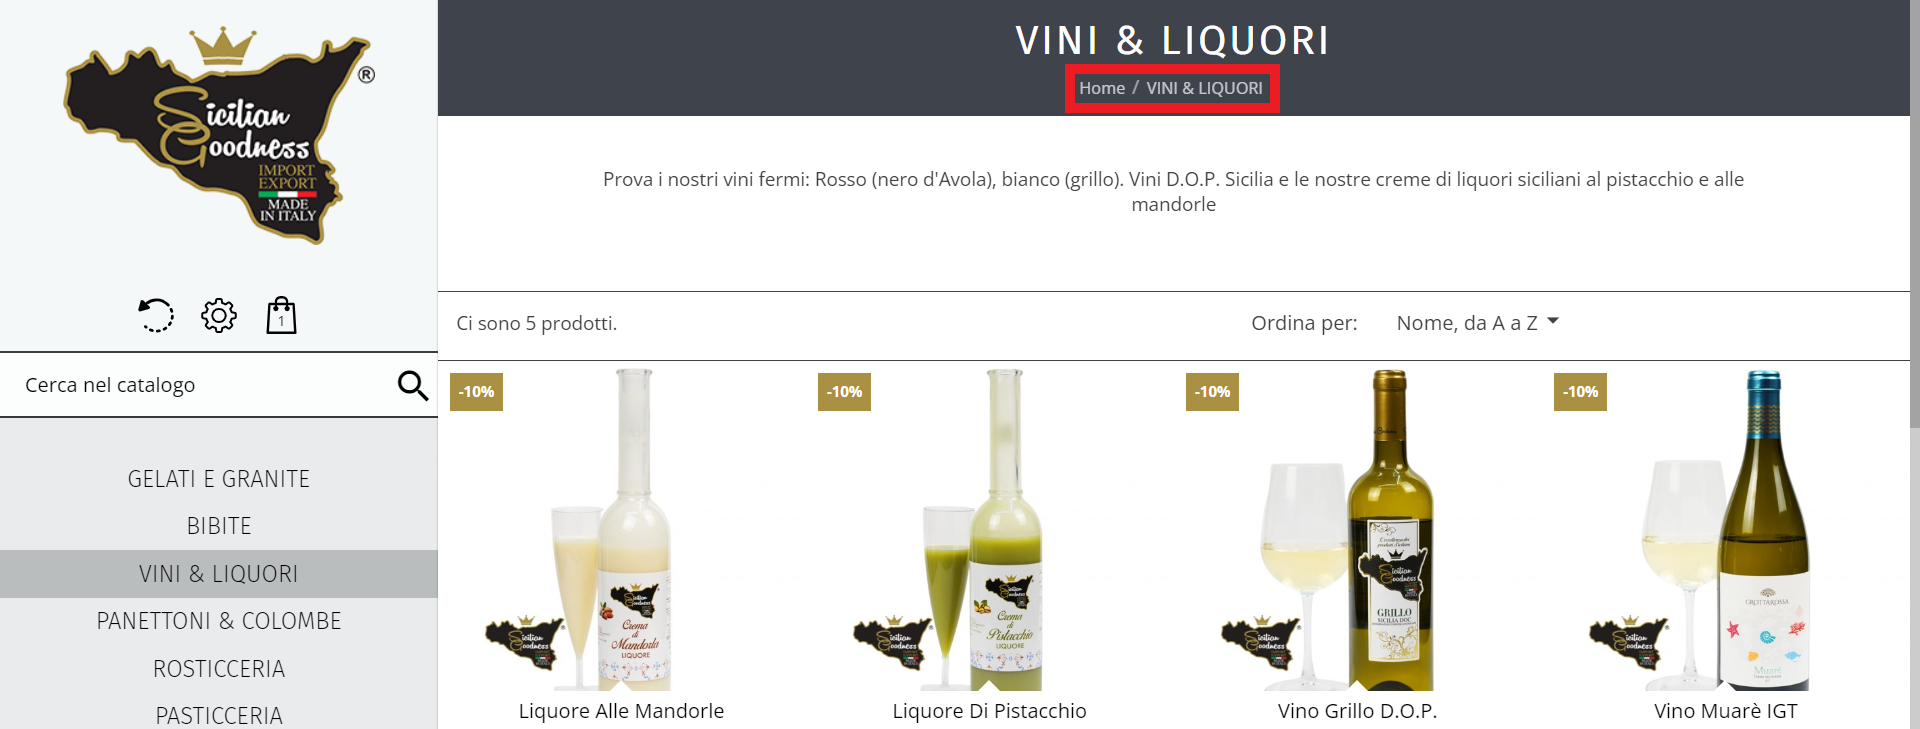
\includegraphics[width=12cm]{Img/bred1.png}
	\caption{Shop Breadcrumb}
\end{figure} 

In particular in this section we'll analyze the page to search the products and the 404 page will be briefly analyzed too. In conclusion we'll analyze the page of a single product (with the analysis of the Ws), as it is the most significant and most visited type of page.

\pagebreak

\subsection{Rest of the pages}
There is a lot of content in this page. In fact, for seeing all the information of the webpage we have to scroll more or less six times.
In the section \textbf{\hyperlink{sho}{First Page}} we analyze better some of the first elements. Now, we brefly see the content.

Immediately, we see that in the center there are all the information about the company(Who axis).

\begin{figure}[H]
	\centering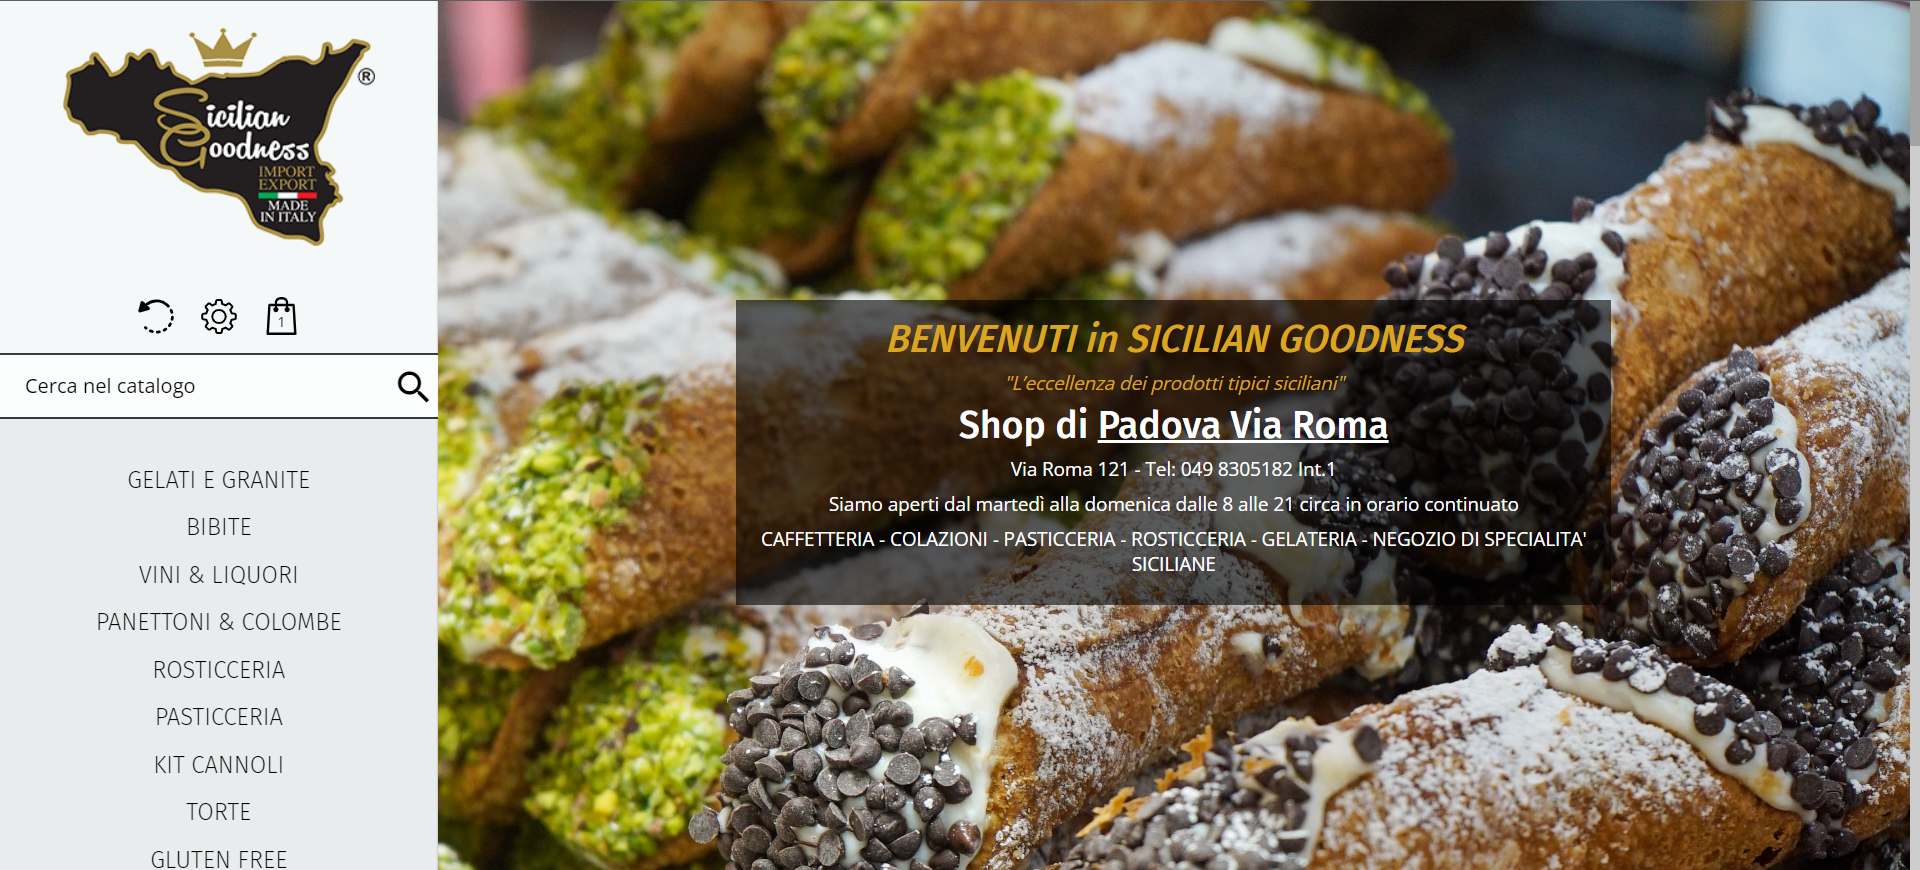
\includegraphics[width=12cm]{Img/con1.png}
	\caption{Content 1}
\end{figure}

In the second scroll we have a video to promote the shop. This can be a good method becuase videos require a low computational effort.

\begin{figure}[H]
	\centering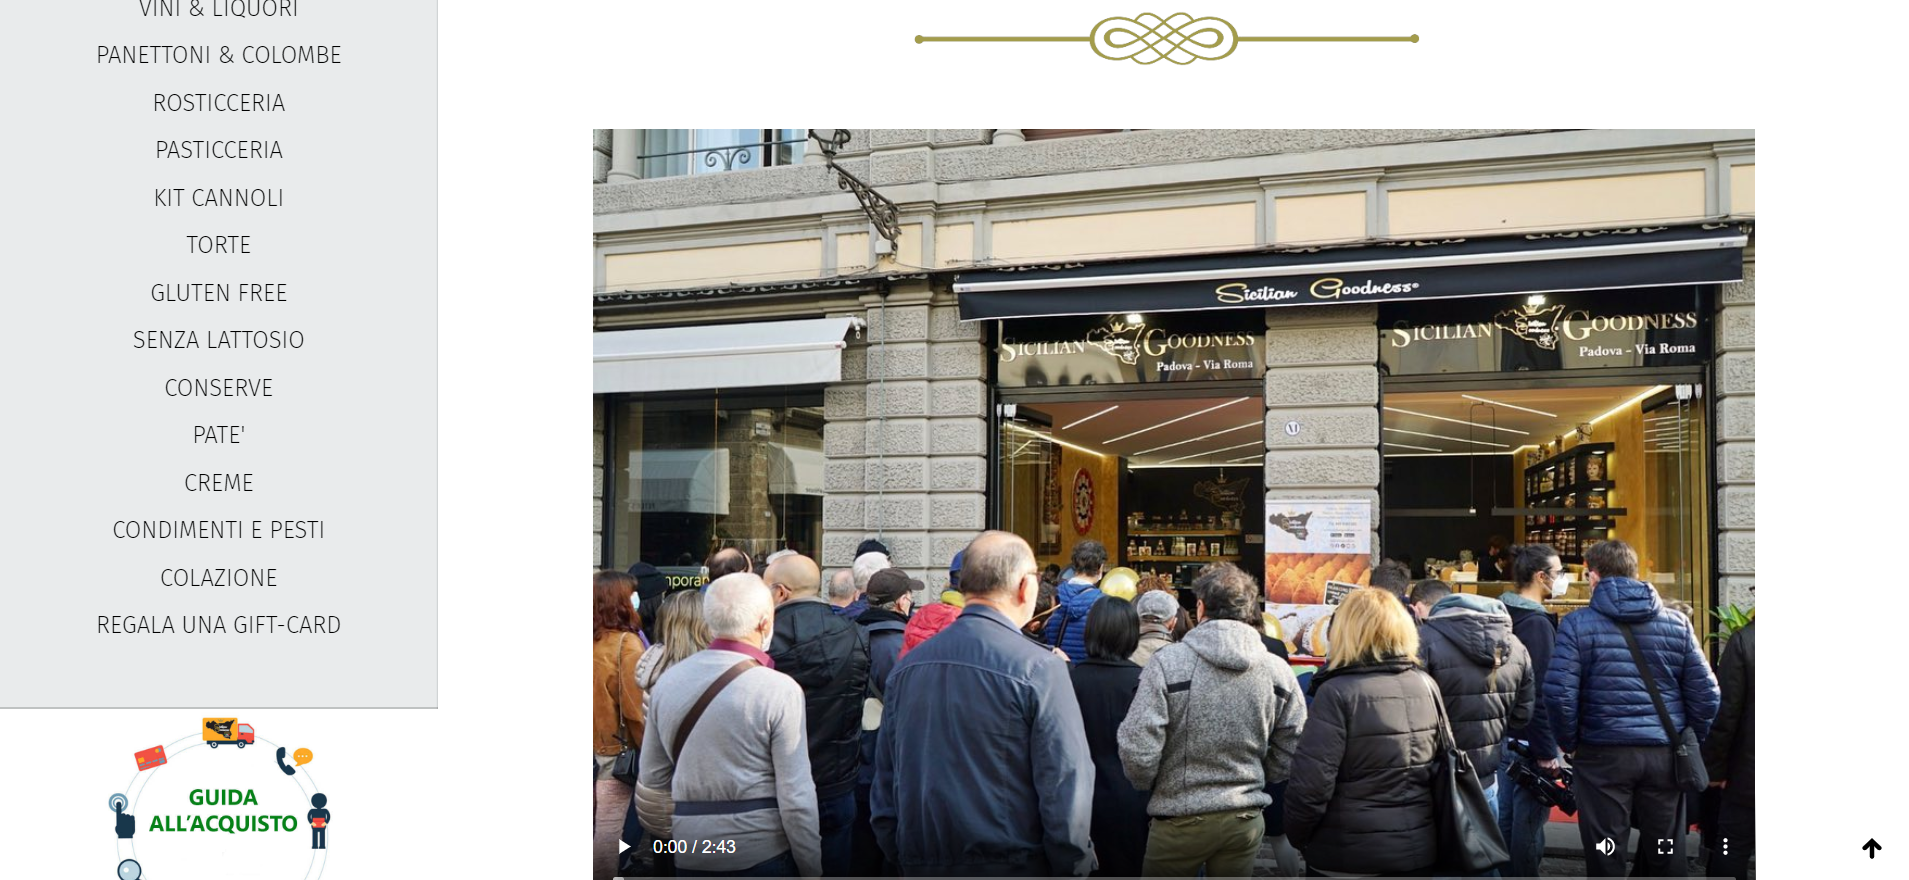
\includegraphics[width=12cm]{Img/con2.png}
	\caption{Content 2}
\end{figure}

\pagebreak

In the third scroll we have some advertisement.

\begin{figure}[H]
	\centering
\includegraphics[width=12cm]{Img/con3.png}
	\caption{Content 3}
\end{figure}

In the fourth scroll we have some popular products in order to help users in the choice.

\begin{figure}[H]
	\centering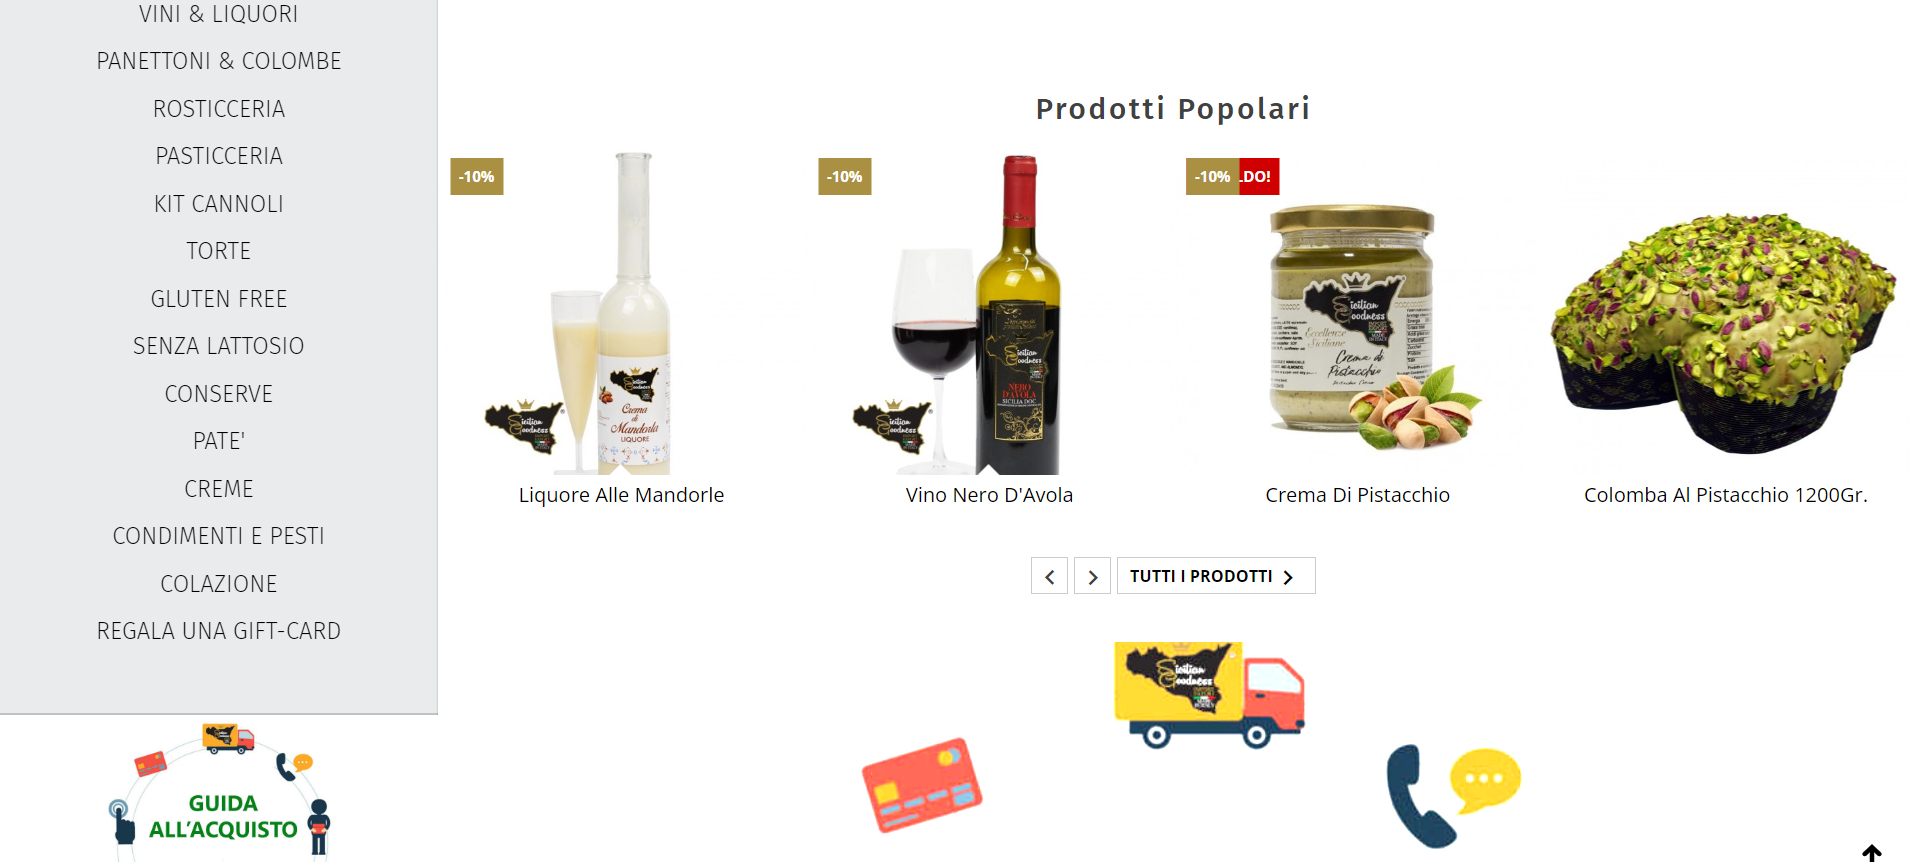
\includegraphics[width=12cm]{Img/con4.png}
	\caption{Content 4}
\end{figure}

In the fifth scroll there is an additional menu to help the user.

\begin{figure}[H]
	\centering
\includegraphics[width=12cm]{Img/con5.png}
	\caption{Content 5}
\end{figure}

In the last scroll we have the footer with all the information.

\begin{figure}[H]
	\centering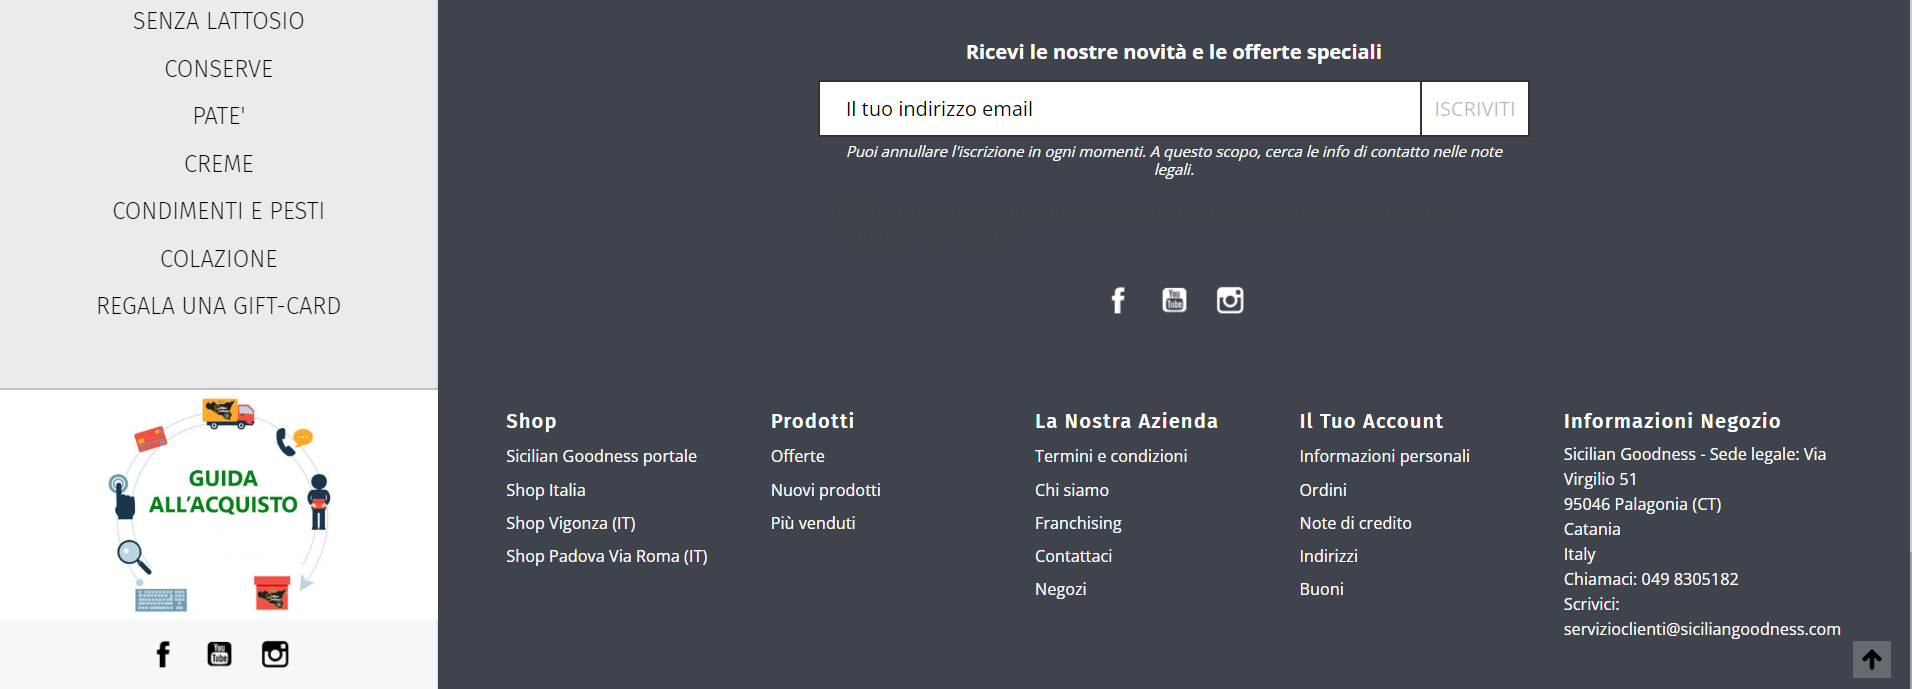
\includegraphics[width=12cm]{Img/con6.png}
	\caption{Content 6}
\end{figure}

\pagebreak

\subsection{First page} \label{sho}
In this page the logo is well situated in the top-left corner of the website.
We don't deeply analyze the Ws but we can see in the image that  mandatory axis are present(Who: in the center, Where: in the center, What: in the left column).

\begin{figure}[H]
	\centering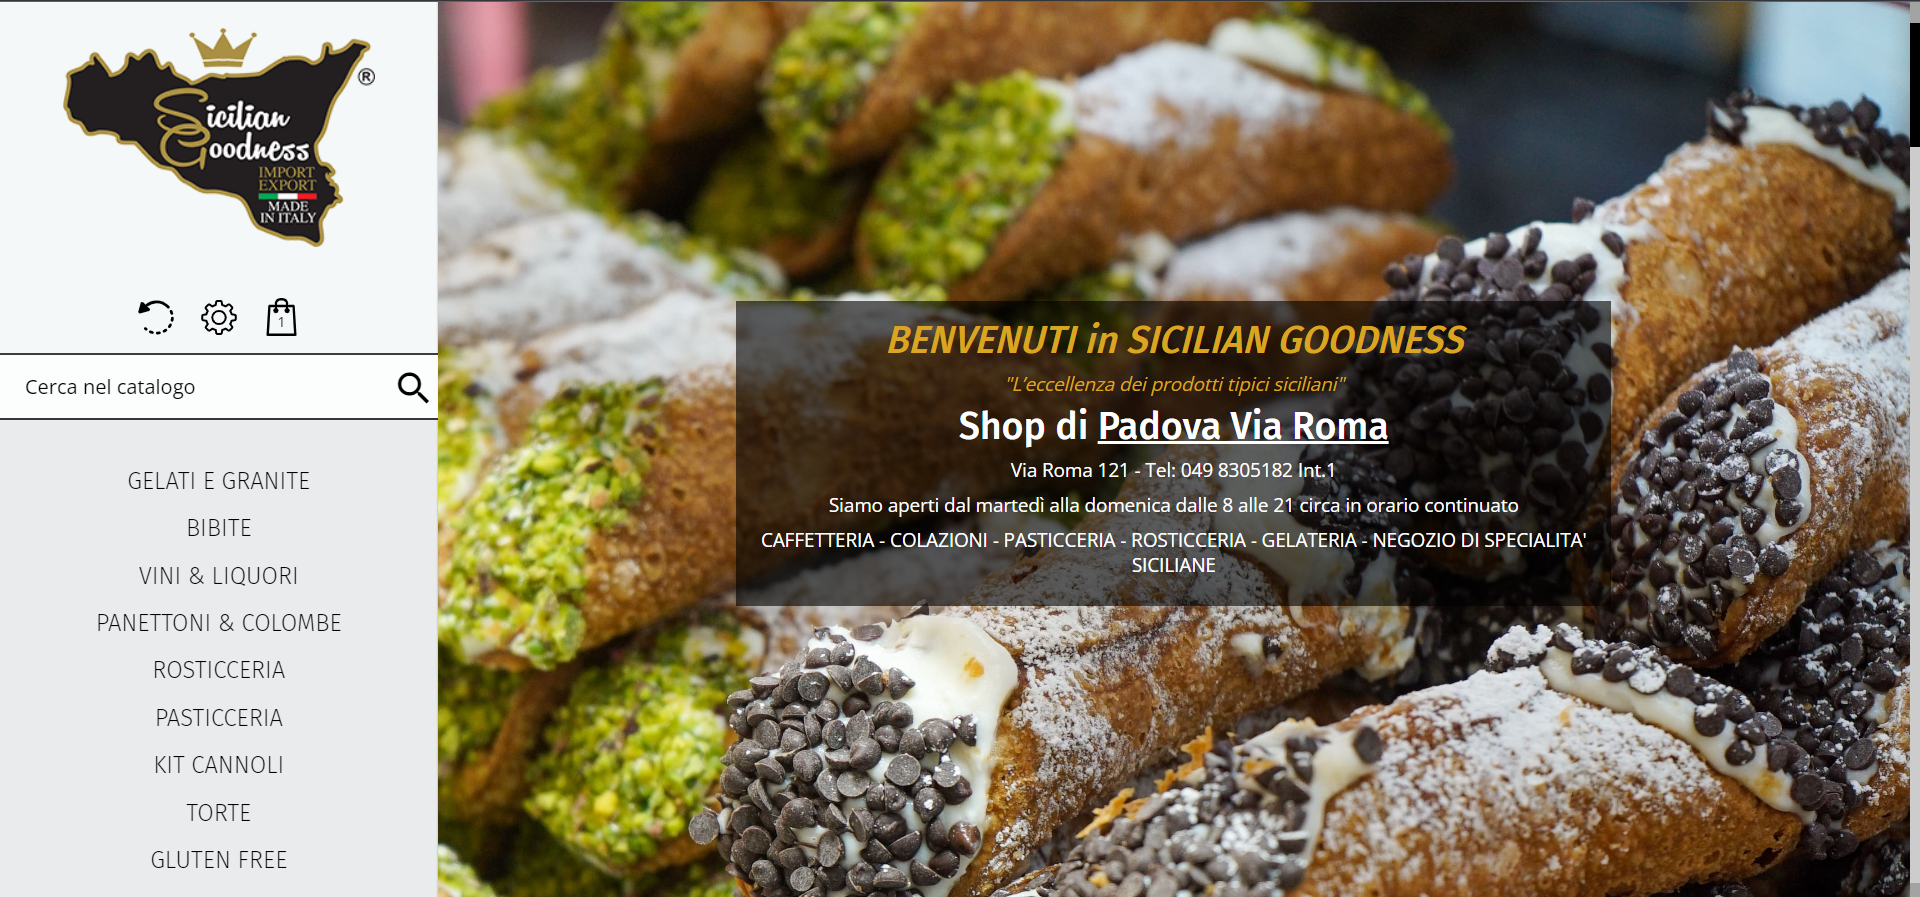
\includegraphics[width=12cm]{Img/Shop.png}
	\caption{Shop page}
\end{figure}

The menu is well structured vertically. In fact, the user can clearly search what he wants. 
Even the underlying menu is well structured. Indeed, whit its design it avoids unwanted clicks.

\begin{figure}[H]
	\centering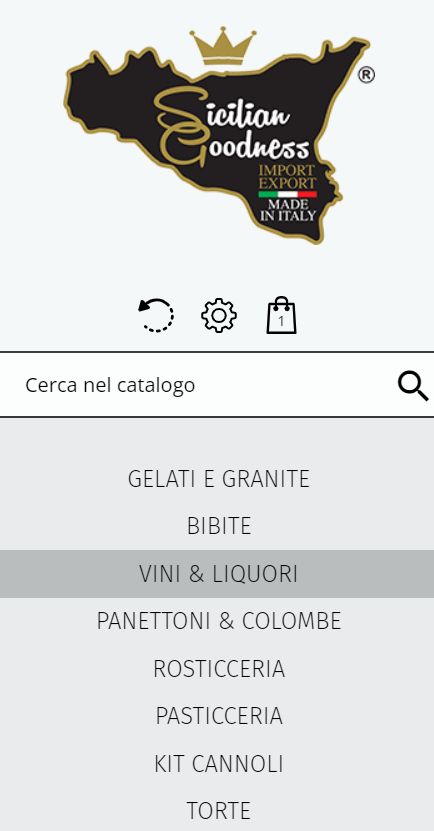
\includegraphics[height=10.5cm, width=7cm]{Img/menushop1.png}
	\caption{Menu Shop page 1}
\end{figure}

\begin{figure}[H]
	\centering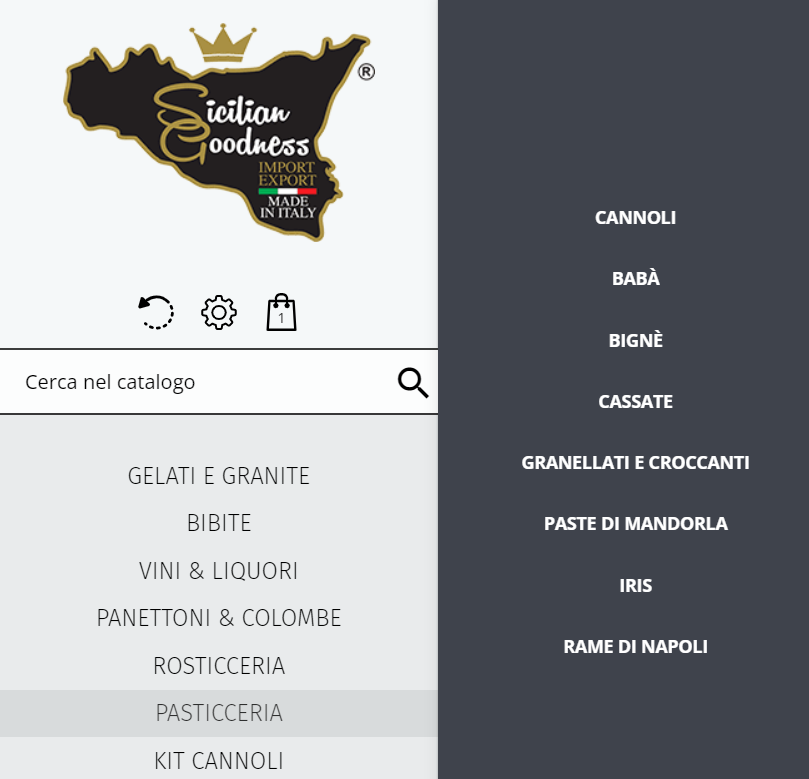
\includegraphics[height=12cm, width=12 cm]{Img/menushop2.png}
	\caption{Menu Shop page 2}
\end{figure}

To reload the page we can click on the logo or in the apposite icon under the logo.
On the right(of the previous icon) we find the registration button/icon. 
This is an other important factor because the registration is not mandatory and is not forced in any way.

\pagebreak

\subsection{Search}
Below these two icons we find the search functionality. 

\begin{figure}[H]
	\centering
\includegraphics[height=12cm, width=10 cm]{Img/search.png}
	\caption{Search functionality}
\end{figure}

It is well structured and located in a good position.
If we use the search functionality, then we can obtain:
\begin{itemize}
	\item the results(Item);
	\item no results.
\end{itemize}

\pagebreak
  
\subsubsection{Item}
In this page we can see that the items are well locate.
Being an e-commerce, prices and products are very important.
We can observe that the website, in order to attract users, uses appropiate colors and good photos.

\begin{figure}[H]
	\centering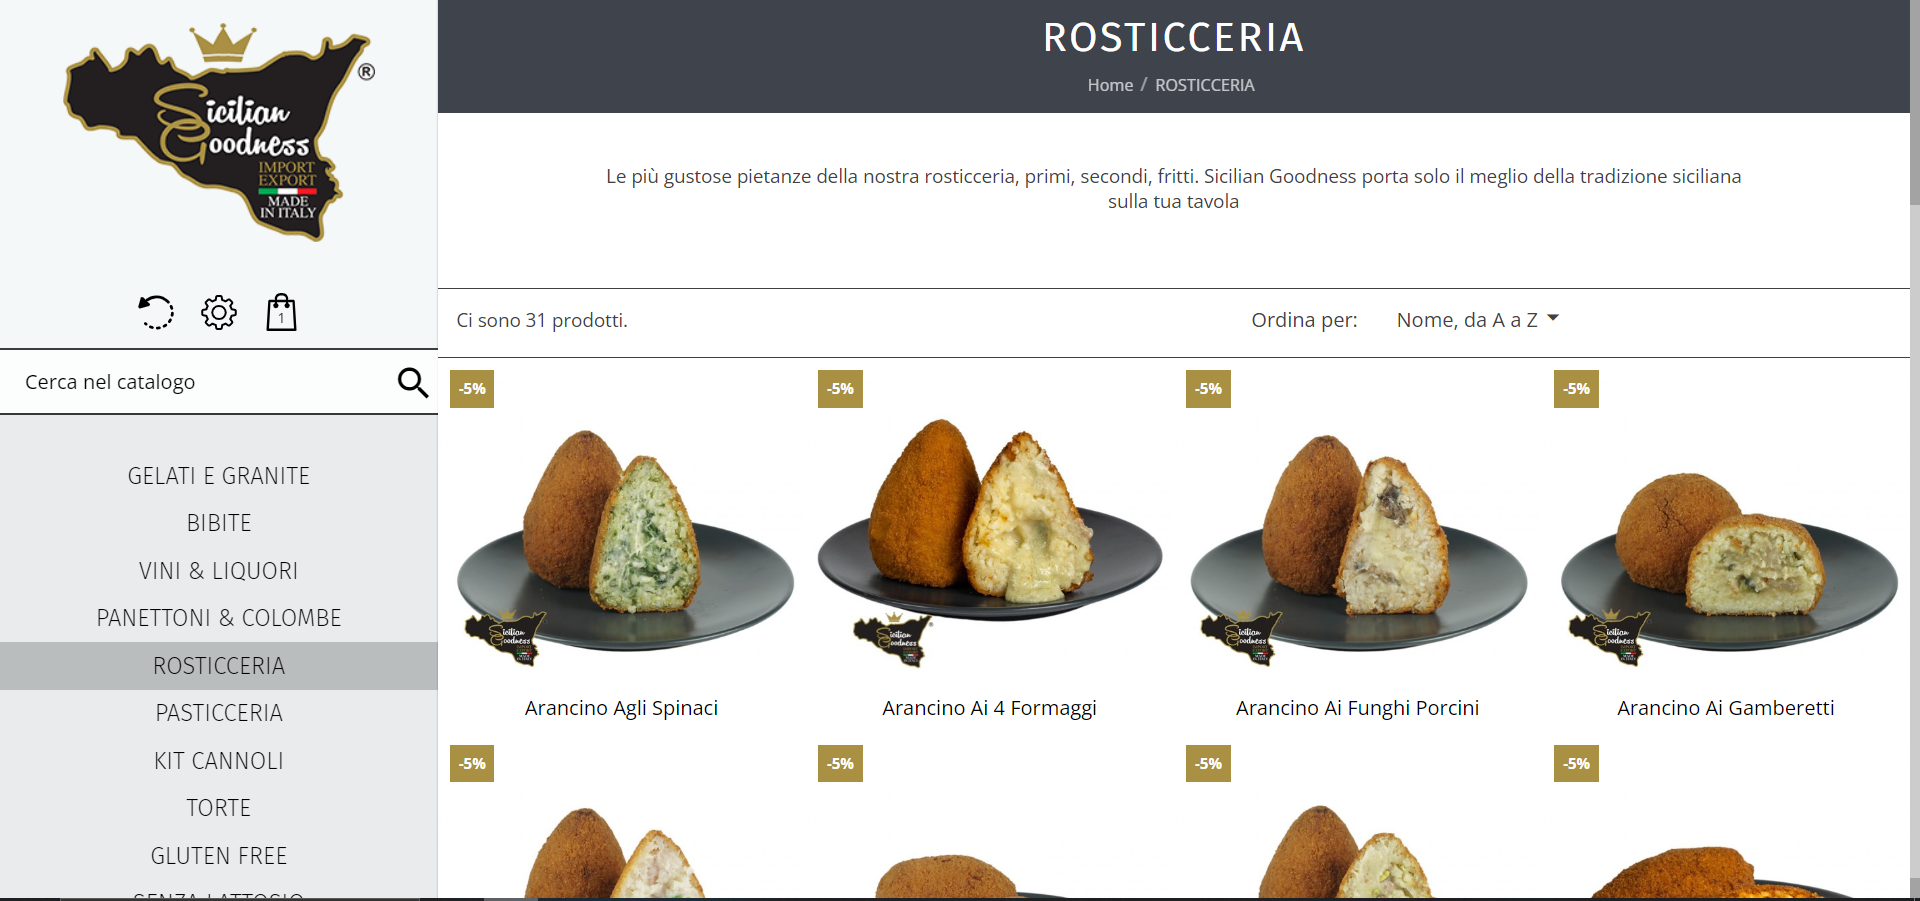
\includegraphics[width=12cm]{Img/product.png}
	\caption{Products}
\end{figure}

In this page we immediately see the percentage of discount but not the price.
The only way to see the price is the hover event and this is not too good. It is better that the price is always visible because it is one of the most important things for a user.
However, The website puts price close to the description and that is good. In addition, an other good thing is that you can see both the price and discounted price.

\begin{figure}[H]
	\centering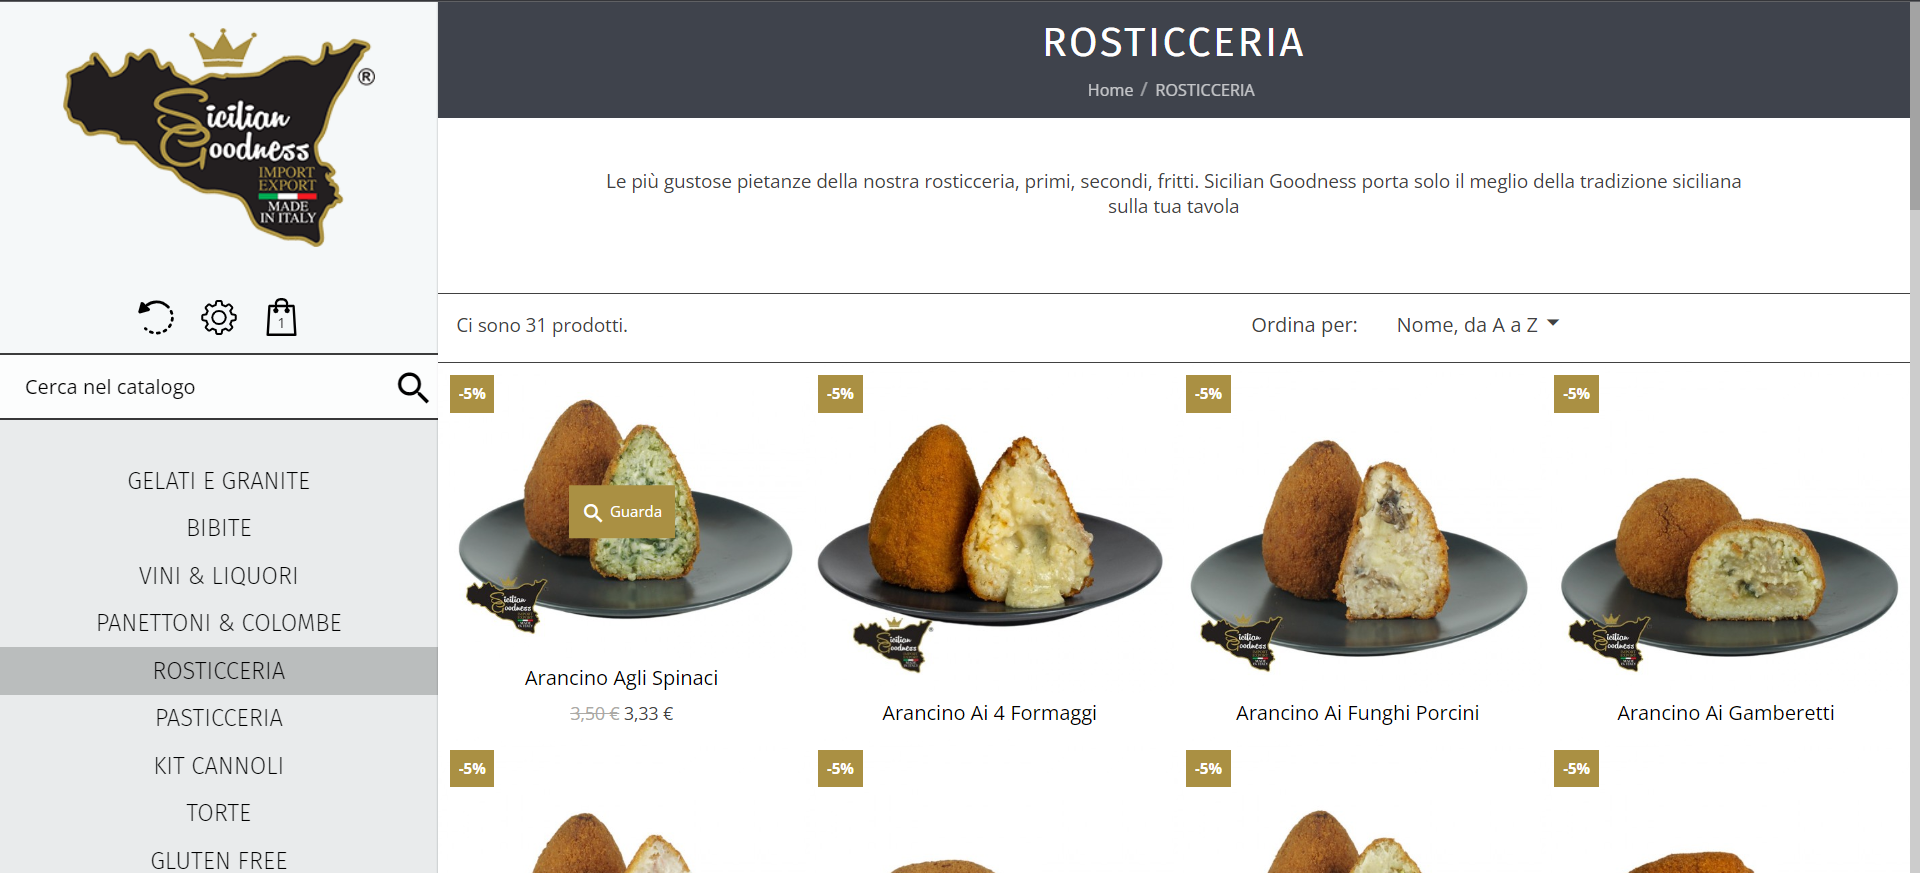
\includegraphics[width=12cm]{Img/price.png}
	\caption{Price}
\end{figure}


\subsubsection{No results}
If a product is searched through the search functionality that is not present within the site, it is displayed a clear error message.
For example we looked for 'milk' but this result doesn't exist. The website provides a good solution even if it not displays a description.

\begin{figure}[H]
	\centering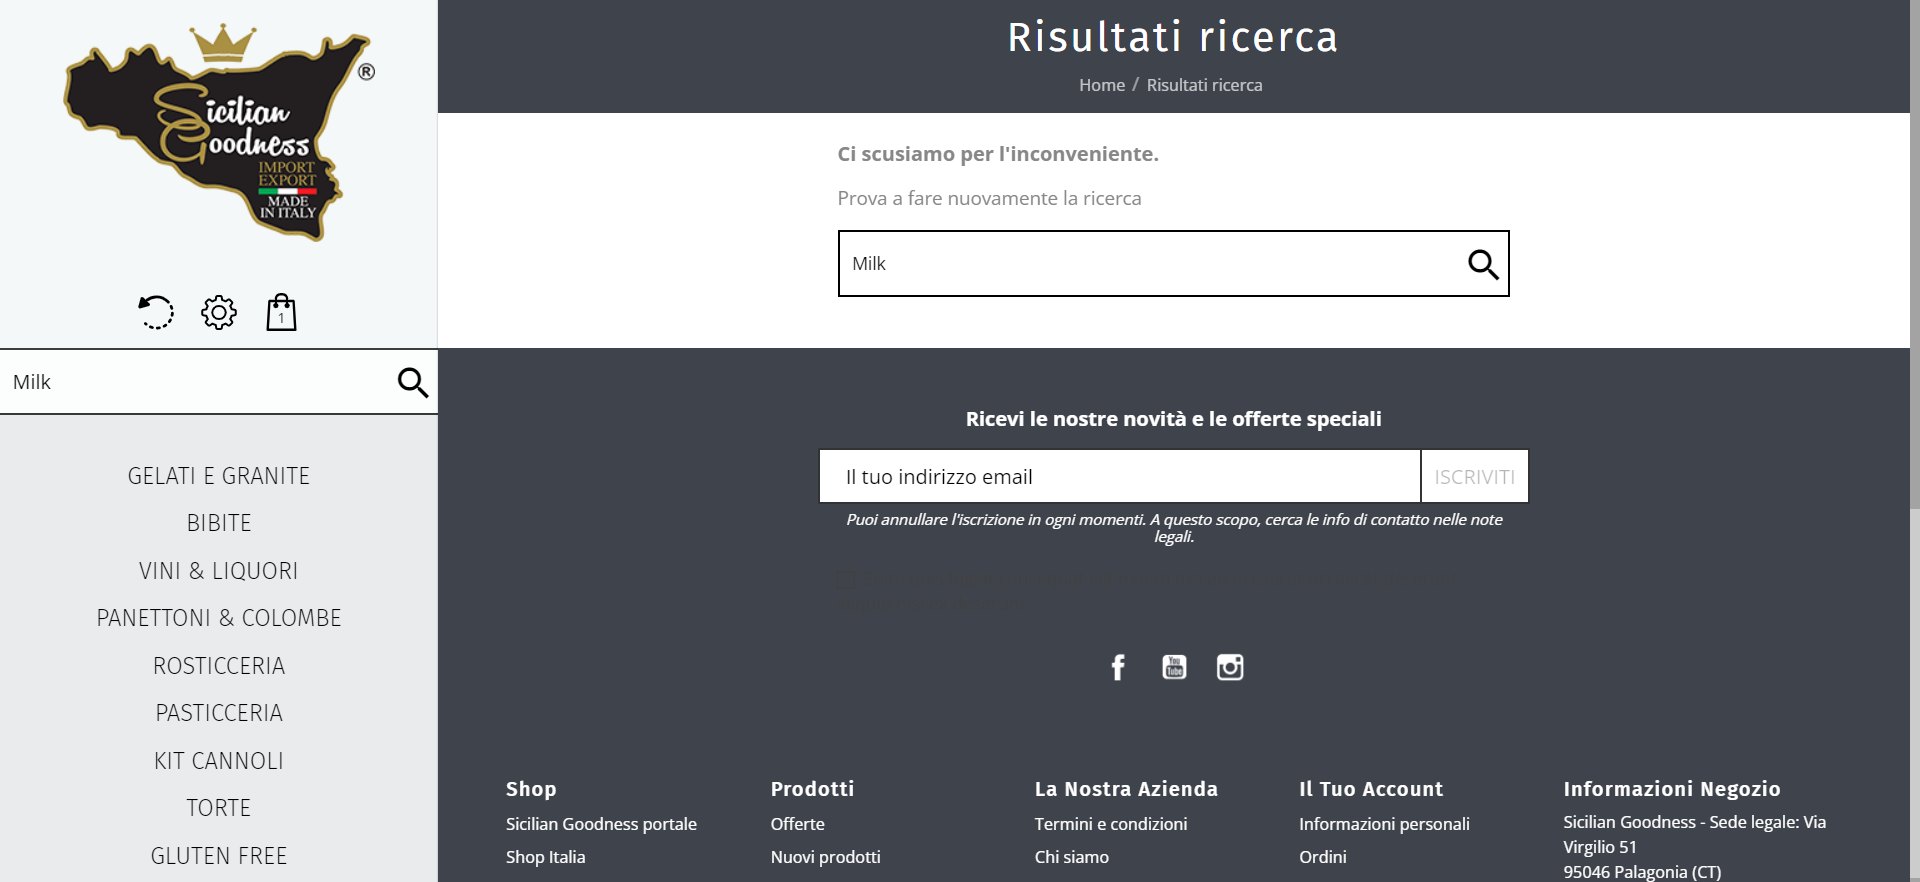
\includegraphics[width=12cm]{Img/noresult.png}
	\caption{No results page}
\end{figure}

\subsection{404}
When the average user ends up on a non-existent page, it needs simple explanations, without the use of technicalities.
If a page is searched through the URL that is not present within the site, it is displayed a clear error message.
For example we looked for \url{https://siciliangoodness.shop/padovaviaroma/vio} but this page doesn't exist. The website provides a good solution telling that the page doesn't exist.

\begin{figure}[H]
	\centering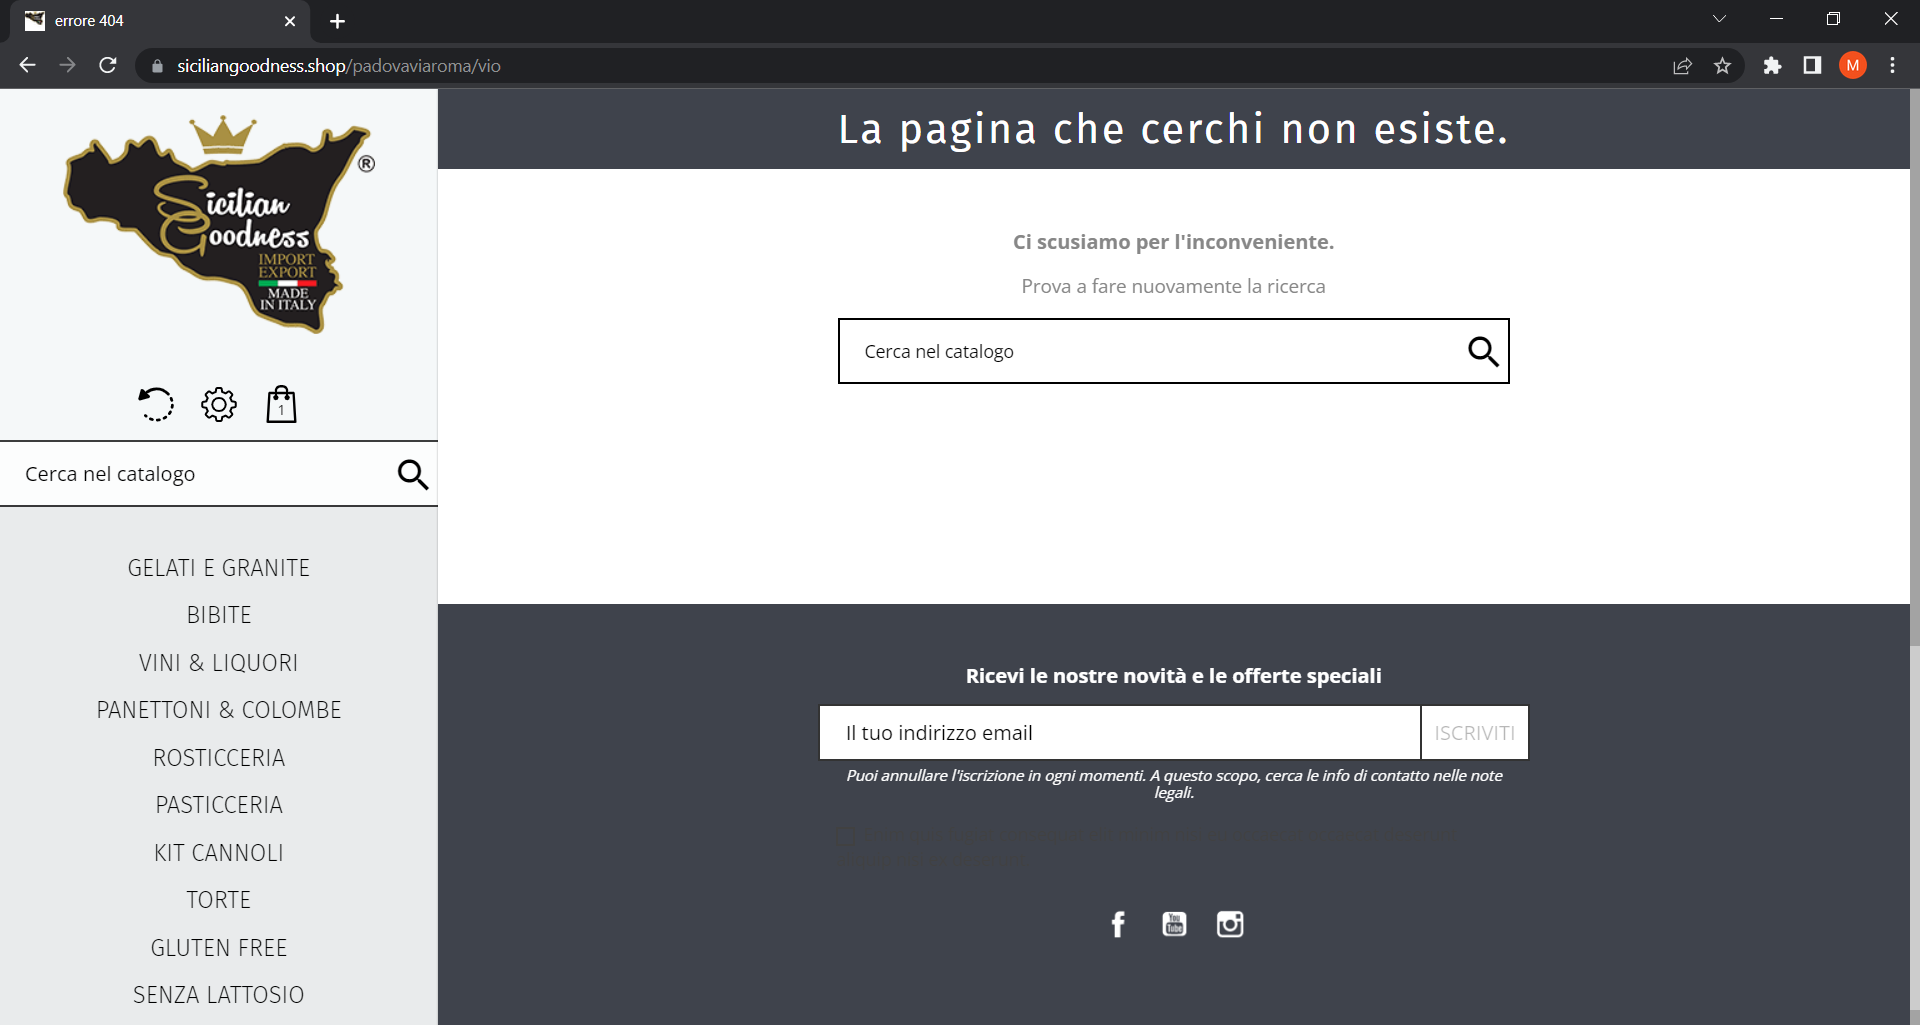
\includegraphics[width=12cm]{Img/404.png}
	\caption{404 page}
\end{figure}

\pagebreak

\subsection{Product}
The page that we analyze is \url{https://siciliangoodness.shop/padovaviaroma/rosticceria/2-arancino-al-pistacchio.html}.

\begin{figure}[H]
	\label{internalpage}
	\centering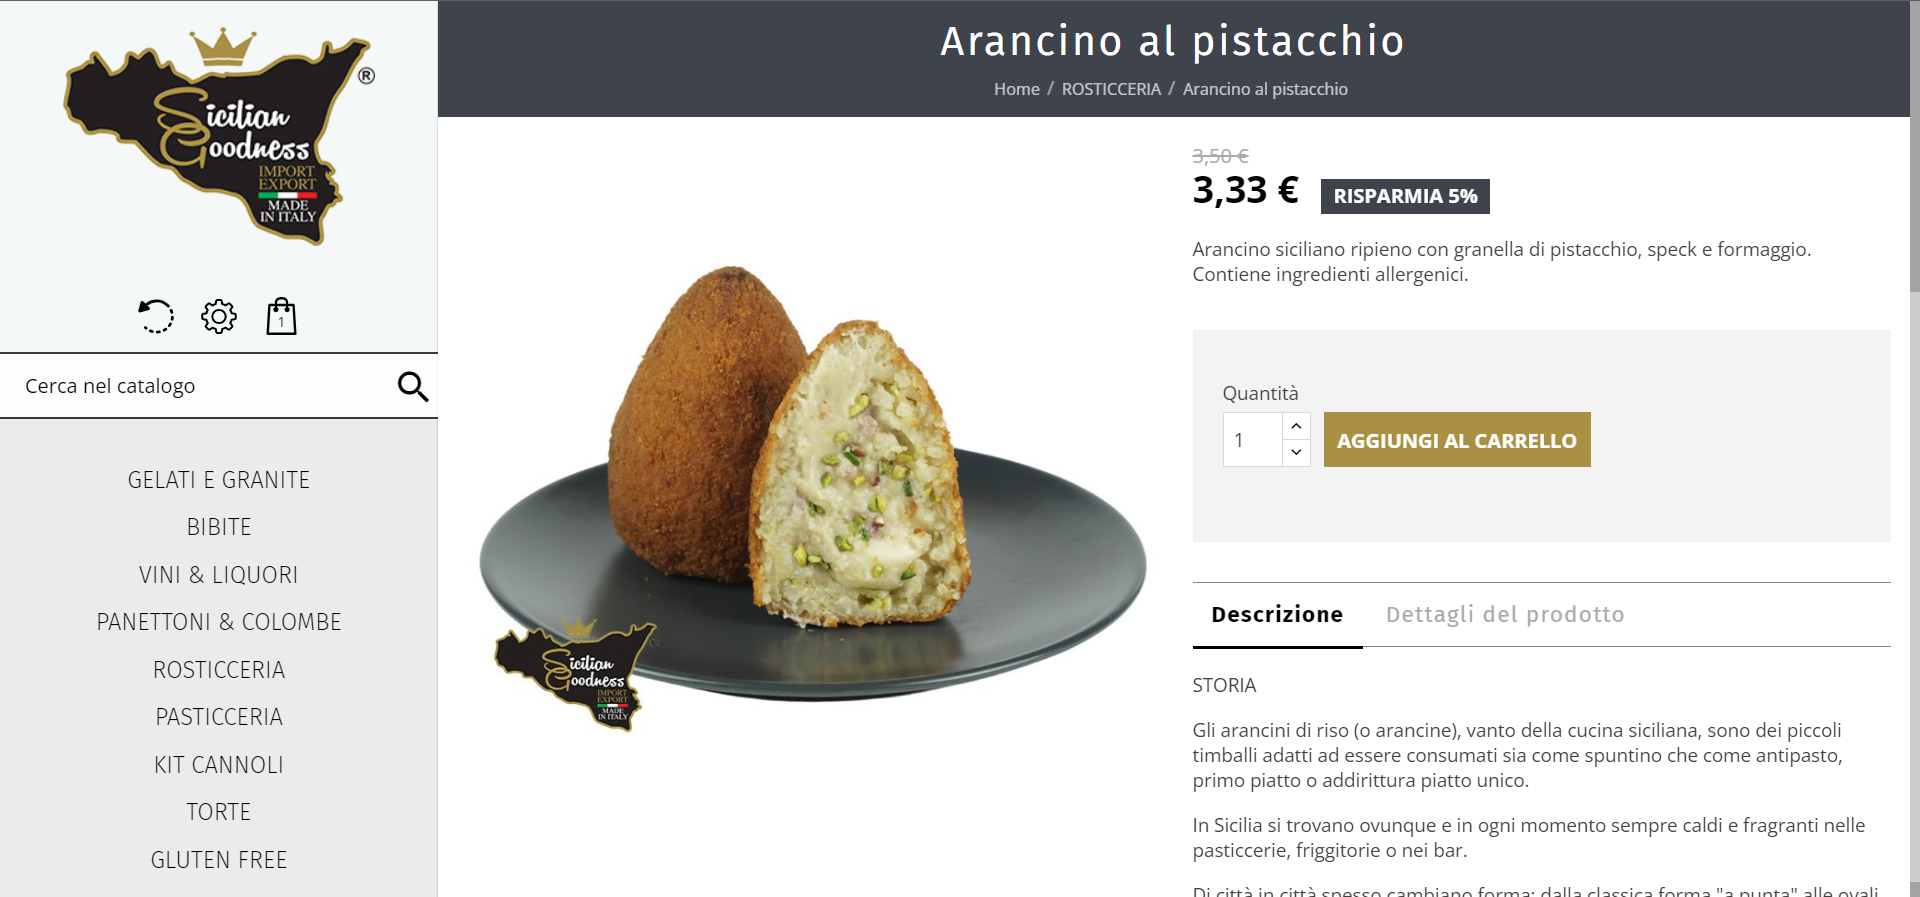
\includegraphics[width=12cm]{Img/internal.png}
	\caption{Internal page}
\end{figure}

Usually, the internal pages do not necessarily have to answer all 6 Ws:
\begin{itemize}
	\item Where: Mandatory;
	\item Who: Mandatory;
	\item What: Mandatory;
	\item When: Optional;
	\item Why: Optional;
	\item How: Optional.
\end{itemize}
As for the homepage to analyze the internal page we analyze the so-called "Six Ws".
This analysis is valid more or less for all the internal pages.

\subsubsection{The Six Ws}

\paragraph{Where}
This axis continues to have a lot of importance in the internal pages since it solves the problem of lost in navigation, allowing you to make it clear context to the user. Location breadcrumbs help to remember the path that users follow. So the Where axis is respected. 

\begin{figure}[H]
	\centering
\includegraphics[width=12cm]{Img/location.png}
	\caption{Location breadcrumb}
\end{figure}

\paragraph{Who}
Also this axis remains mandatory in internal pages, but it is sufficient to display the company logo, which Sicilian Goodness does by keeping it in the upper left corner.

\paragraph{What}
This axis remains mandatory and the presence of references to food make it clear that the theme are Sicilian procuts. The title and description help to understand the type of product.

\paragraph{When}
It is optional and this page doesn't contain any temporal reference.

\paragraph{Why}
This axis, even if it is optional, it is described very well in the section 'STORIA' as we can see in the \textbf{\hyperlink{internalpage}{Figure 35}}

\paragraph{How}
This axis is optional but it is present. In fact the search functionality is always available and we have also some tools in the footer.

\subsubsection{Cart}

The tabular display of the inserted products is very clear, where you can see the total price and the price, the discounted price with the percentage and the description of the single product. Moreover the site offers the possibility to increase the number of products or to remove items that you no longer want.

\begin{figure}[H]
	\centering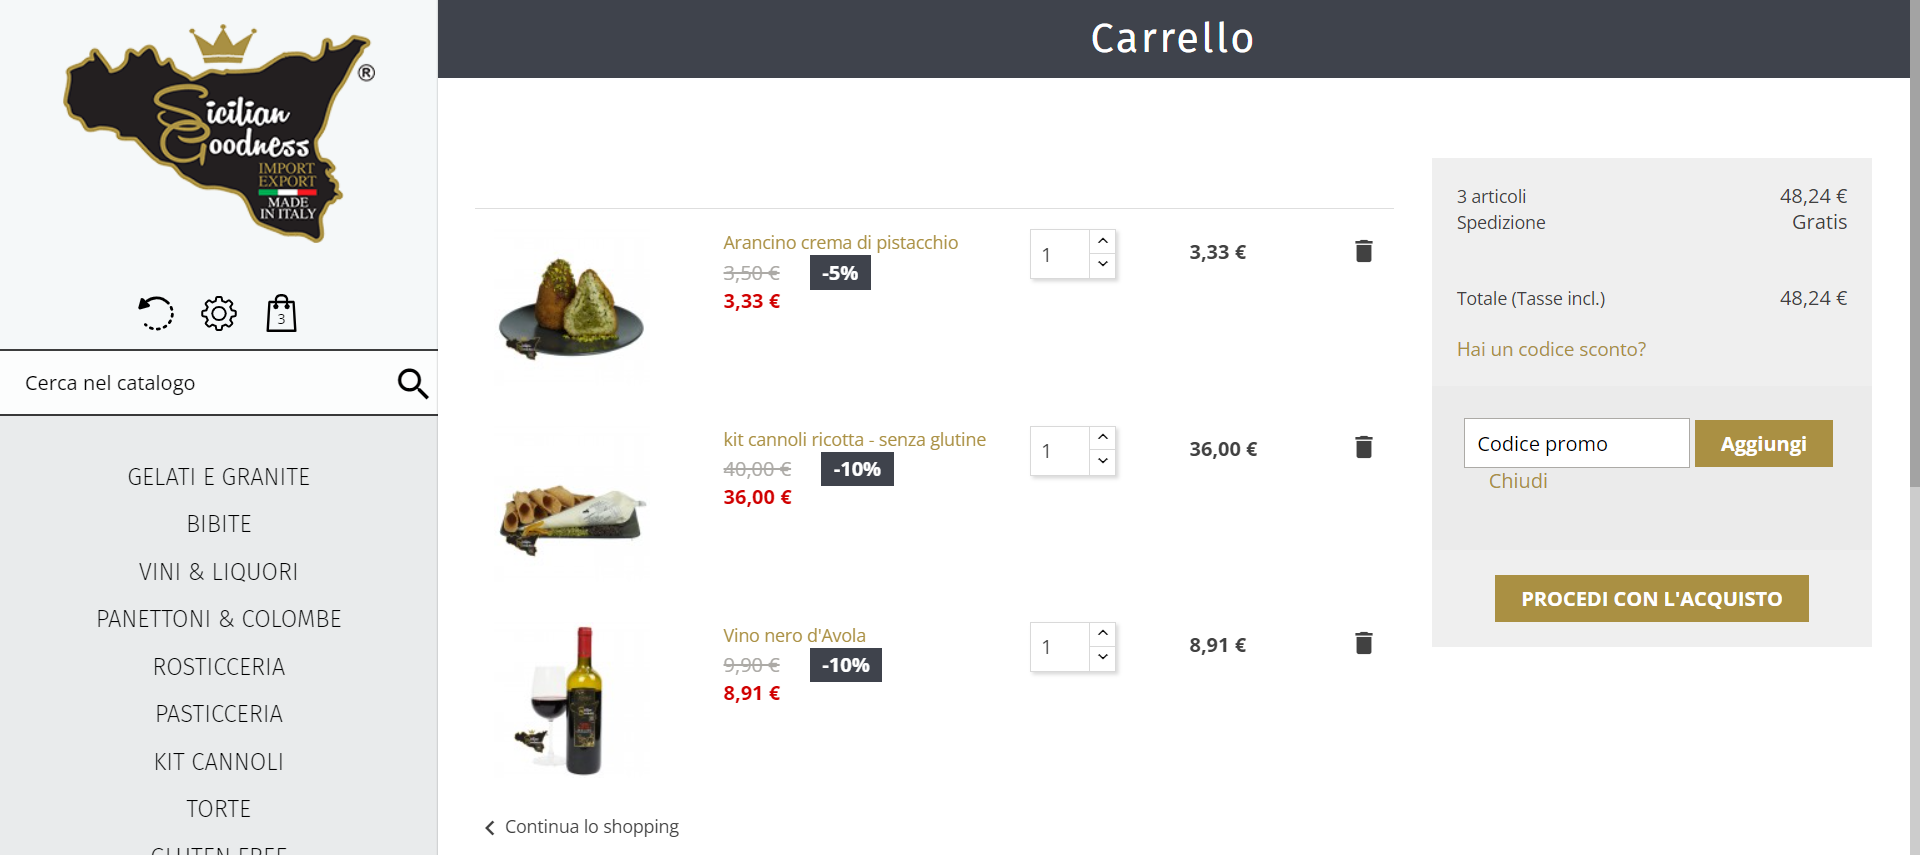
\includegraphics[width=12cm]{Img/cart.png}
	\caption{Cart}
\end{figure}

\pagebreak
\section{Advertising}


\pagebreak
\section{Evaluation}
One problem encoutered is in the homepage. There are the icons of the Play and App Store but this two links don't work and doing this the website risks to lose the trust of the user and his available time.
However, the homepage has a simple and clear layout that separates the contents very well and the internal pages do the same.
The structure is simple but well organised, after a few clicks the user has a clear idea of where to look for what he needs. 
Moreover the search functionality helps the user if he doesn't know where what he's looking for is. 
After all the considerations made in the document, Sicilian Goodness is a good site for all types of users. It doesn't commit serious usability errors and according to the analysis of the 6 Ws it provides all the information a user needs when he navigates a site. \newline
In conclusion, the evaluation is positive and the final grade is 8/10.


\section{Pictures}

\pagebreak


\end{document}